\documentclass[10pt,twocolumn,letterpaper]{article}

\usepackage{iccv}
\usepackage{times}
\usepackage{epsfig}
\usepackage{graphicx}
\usepackage{amsmath}
\usepackage{amssymb}
\usepackage{caption}
\usepackage{subcaption}


% Include other packages here, before hyperref.

% If you comment hyperref and then uncomment it, you should delete
% egpaper.aux before re-running latex.  (Or just hit 'q' on the first latex
% run, let it finish, and you should be clear).
\usepackage[breaklinks=true,bookmarks=false]{hyperref}

\iccvfinalcopy % *** Uncomment this line for the final submission

% Pages are numbered in submission mode, and unnumbered in camera-ready
\ificcvfinal\pagestyle{empty}\fi

\begin{document}

%%%%%%%%% TITLE
\title{Differentiable Point-Based Radiance
Fields for Efficient View Synthesis with
Imperfect Masks}

\author{Jason C. Yuan\\
Department of Computer Science, Princeton University\\
% Institution1 address\\
{\tt\small jcyuan@princeton.edu}
% For a paper whose authors are all at the same institution,
% omit the following lines up until the closing ``}''.
% Additional authors and addresses can be added with ``\and'',
% just like the second author.
% To save space, use either the email address or home page, not both
% \and
% Second Author\\
% Institution2\\
% First line of institution2 address\\
% {\tt\small secondauthor@i2.org}
}

\maketitle
% Remove page # from the first page of camera-ready.
\ificcvfinal\thispagestyle{empty}\fi

%%%%%%%%% ABSTRACT
\begin{abstract} 
% brief synopsis of the project
Differentiable point-based radiance fields is an alternative algorithm to Neural Radiance Fields to perform novel view synthesis. Crucially, this algorithm relies on the use of object-background masks during training. In this work, we empirically demonstrate the negative effect of imperfect masks on this algorithm's render quality through a simulation of mask corruption. We then propose a two part modification to the algorithm to enable it to handle less-than-perfect masks. We demonstrate quantitatively and qualitatively that our proposed solution has high render quality even with imperfect masks. 

\end{abstract}
%%%%%%%%% BODY TEXT
\section{Introduction}

\let\thefootnote\relax\footnotetext{Code available at \url{https://github.com/jasony123123/point-radiance}.}

% motivate your approach here and situate your work in a broader context of existing neural rendering work that we reviewed in the course.

Novel view synthesis is the task of generating new views of a given object given a collection of training views. The canonical solution to this problem is Neural Radiance Fields (NeRF) \cite{mildenhall2020nerf}, which models the scene as a continuous radiance field using a MLP. However, NeRF is extremely slow to train and render. The authors in \cite{zhang2022differentiable} propose an alternative algorithm: differentiable point-based radiance fields. This approach represents a scene using a 3d point cloud with radiance parameters. This algorithm achieves near state of the art performance on the novel view synthesis task with orders of magnitude less training time, inference time, and memory requirement.

The initialization of the point cloud plays a crucial role in the differentiable point-based radiance field algorithm. A well-executed initialization greatly facilitates the optimization routine in generating a final point-cloud representation of superior quality. This algorithm takes an intuitive approach to achieve this by leveraging a foreground-background mask within the training data. Specifically, points are only initialized if they are consistent with all the masks.

In real world applications, the assumption of an accurate mask may not hold. For example, many real world scenes will not even have a mask provided. Thus, in practice the mask will be generated using a segmentation network or using the depth data of RGBD images. In either case, such masks will have imperfections and not-necessarily be multi-view consistent.

In this work, we are interested in addressing the problem of decent-but-imperfect masks for the differentiable point-based radiance field algorithm. To summarize our contributions:

\begin{itemize}
    \item We develop a method to simulate imperfect masks by adding a small amount of noise. We then empirically characterize the decrease in render quality of the algorithm on imperfect masks.
    \item We propose a two step solution to restore the performance of this algorithm even on imperfect masks. We quantitatively and qualitatively demonstrate the proposed solution enables differentiable-point-based-radiance-field to handle imperfect masks successfully.
\end{itemize}

\section{Related Work}

% review relevant related work and include citations, cite at least 10 related papers here.

A wide variety of algorithms have been proposed for the novel view synthesis task, which have differing requirements in terms of masks. The algorithm that is the study of this paper was introduced in \cite{zhang2022differentiable}. 

In \cite{mildenhall2020nerf}, the authors introduce NeRF which uses a MLP to model the scene. It is orders of magnitude slower than \cite{zhang2022differentiable} but masks are not needed. \cite{reiser2021kilonerf} present a modification to NeRF where a MLP is split into many smaller MLPs to accelerate rendering and also requires no masks. \cite{kondo2021vaxnerf} propose an addition to NeRF using masks to reduce NERF network evaluations. \cite{Garbin21arxiv_FastNeRF} modifies NeRF to use a factorized expression, increasing the inference speed without requiring masks.

Plenoxels are a non-MLP approach introduced in \cite{yu_and_fridovichkeil2021plenoxels} that are very fast but require significant memory and a mask to determine what volume to optimize. An alternative point-cloud based model is given in \cite{Rakhimov_2022_CVPR}, but likewise requires training data to be masked. \cite{Lassner_2021_CVPR} is another rendering technique that uses COLMAP to get a depth map instead of a mask.

Regularization of render outputs has also been used as a technique to reduce artifacts. \cite{jain2022zeroshot} regularizes opacity near the camera by adding a loss term to maximize transmittance (\ie transparency) in the near plane. \cite{yang2023freenerf} uses a penalty on the sum of densities near the camera to reduce floaters. Both techniques leverage the inductive bias that the space near the camera should generally be free of occlusions.

\section{Method}

% Describe your method and approach here

\subsection{Differentiable Point-Based Radiance Fields}

The input of this algorithm is a viewing direction represented with camera intrinsic and extrinsic parameters $R, t, M$. The output is a 2d RGB image of the scene from that view. For a detailed explanation, refer to \cite{zhang2022differentiable}. The pipeline is given in Figure \ref{fig:model_1to6}.

\begin{figure*}
    \centering
    \begin{subfigure}[b]{0.32\textwidth}
        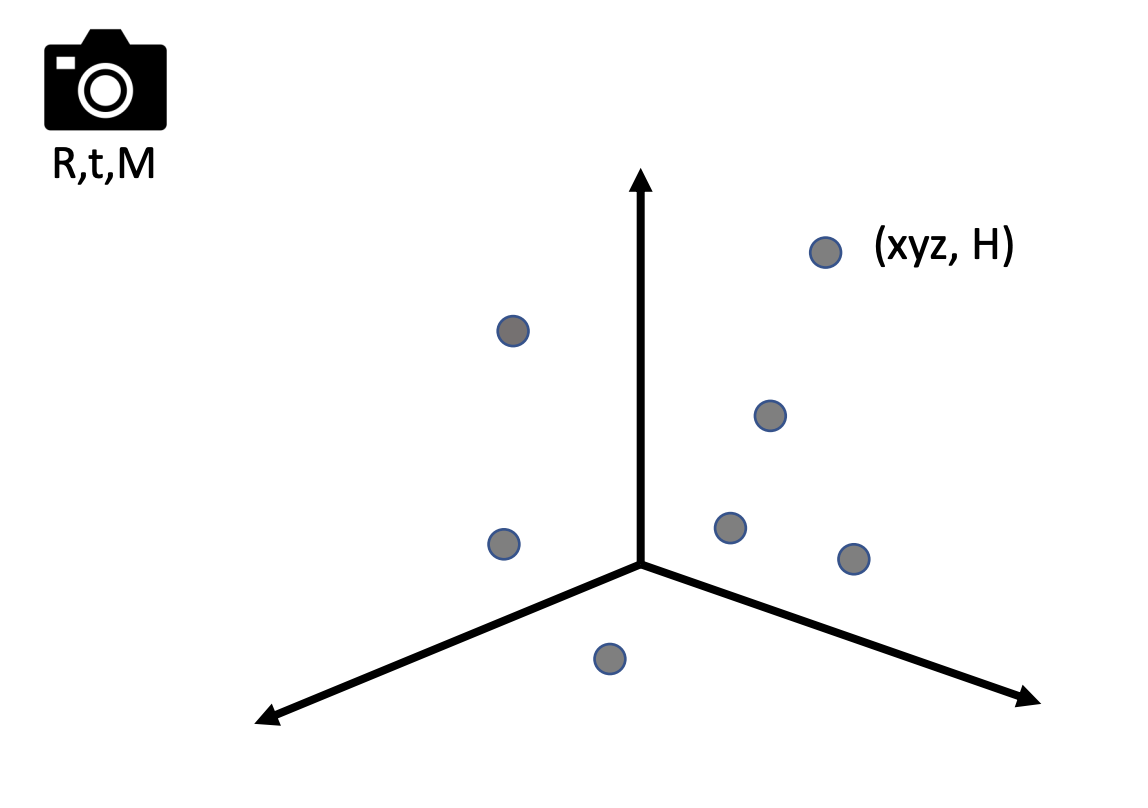
\includegraphics[width=\textwidth]{figures/model_1.png}
        \caption{Model is point-cloud with $(x, y, z, H)$ and a input view $R, t, M$. }
        \label{fig:model_1}
    \end{subfigure}
    \hfill
    \begin{subfigure}[b]{0.32\textwidth}  
        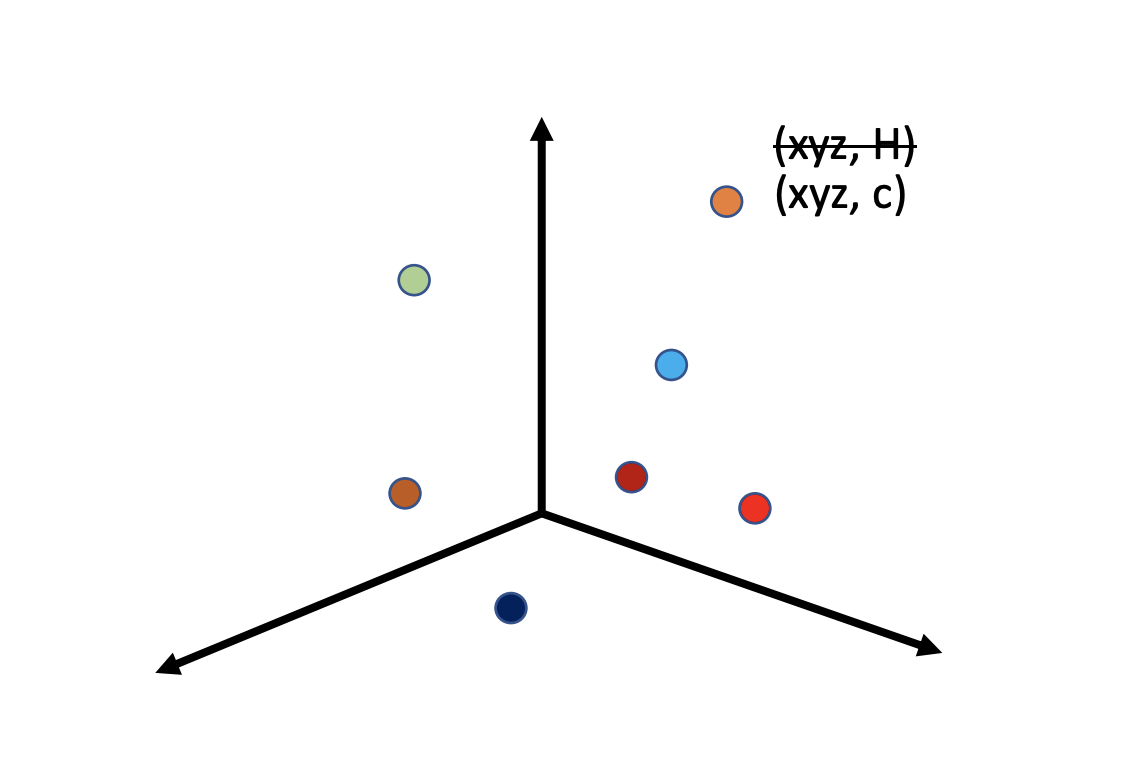
\includegraphics[width=\textwidth]{figures/model_2.png}
        \caption{View-dependent color $c$ can be computed for each point. }
        \label{fig:model_2}
    \end{subfigure}
    \hfill
    \begin{subfigure}[b]{0.32\textwidth}  
        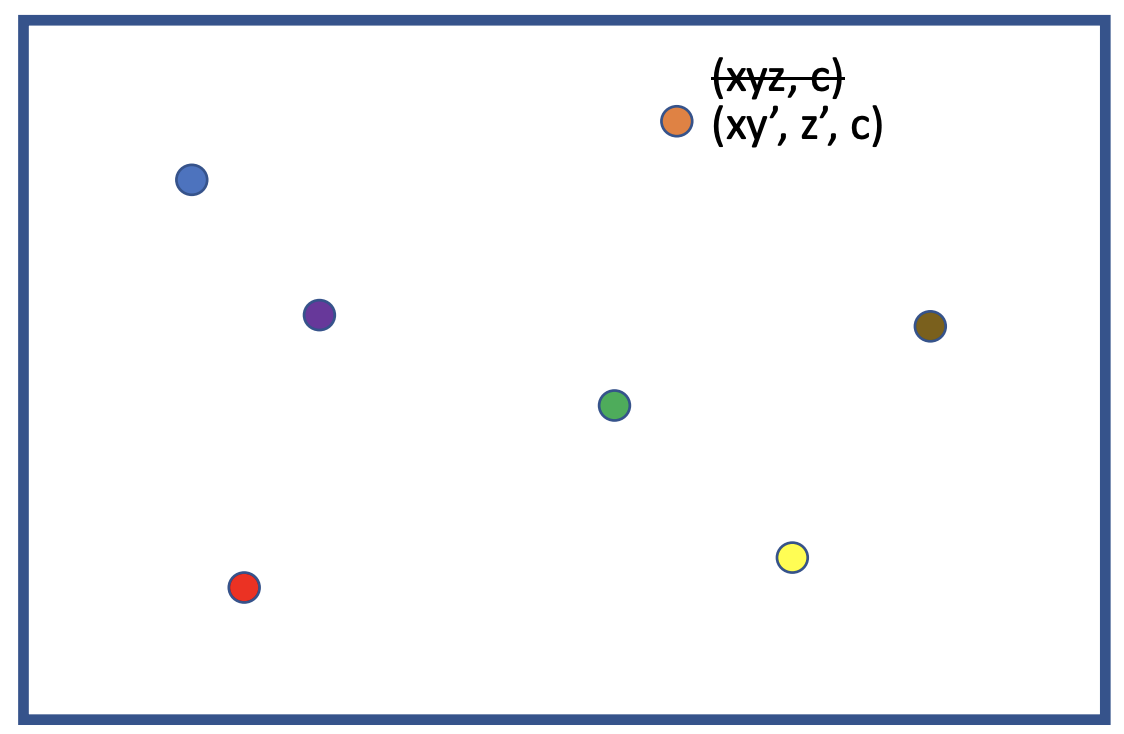
\includegraphics[width=\textwidth]{figures/model_3.png}
        \caption{The 3d point cloud is projected to 2d (plus depth) using the view-direction. }
        \label{fig:model_3}
    \end{subfigure}
    \hfill
    \vskip\baselineskip
    \begin{subfigure}[b]{0.32\textwidth}
        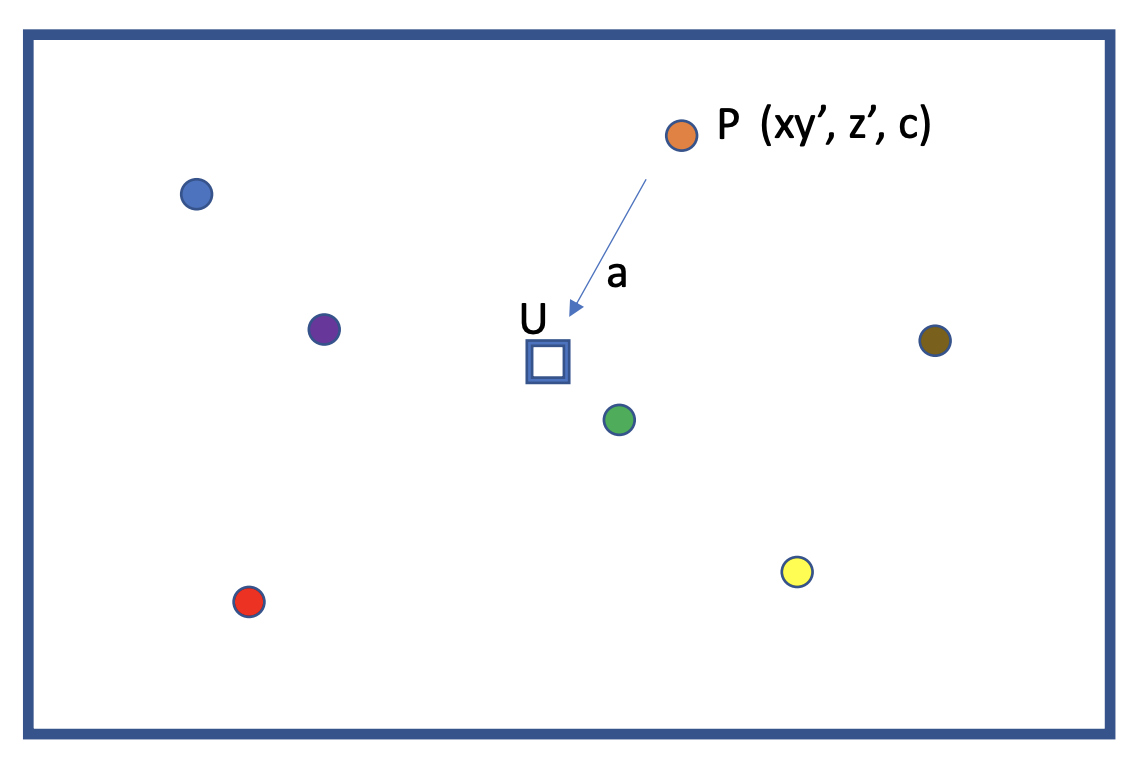
\includegraphics[width=\textwidth]{figures/model_4.png}
        \caption{The $\alpha$ density of a point $P$ on a pixel $U$ is given by a Gaussian kernel. }
        \label{fig:model_4}
    \end{subfigure}
    \hfill
    \begin{subfigure}[b]{0.32\textwidth}  
        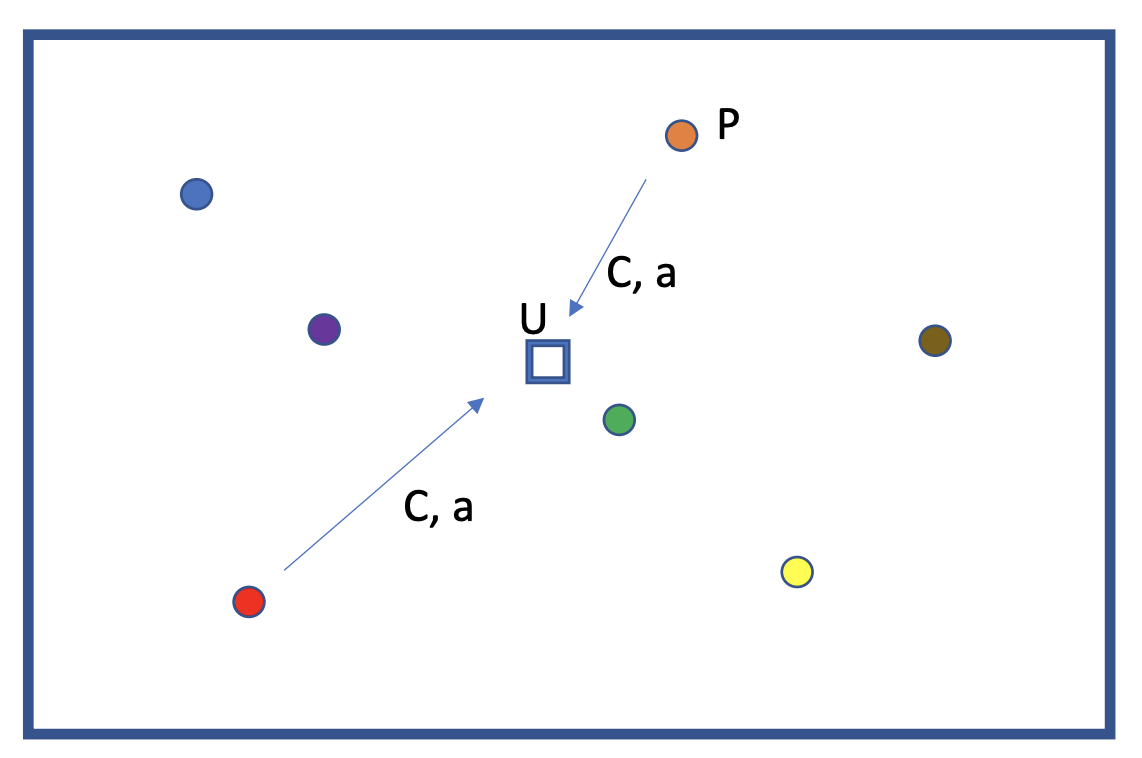
\includegraphics[width=\textwidth]{figures/model_5.png}
        \caption{Every point contributes a color $c$ and density $\alpha$ to every pixel $U$}
        \label{fig:model_5}
    \end{subfigure}
    \hfill
    \begin{subfigure}[b]{0.32\textwidth}  
        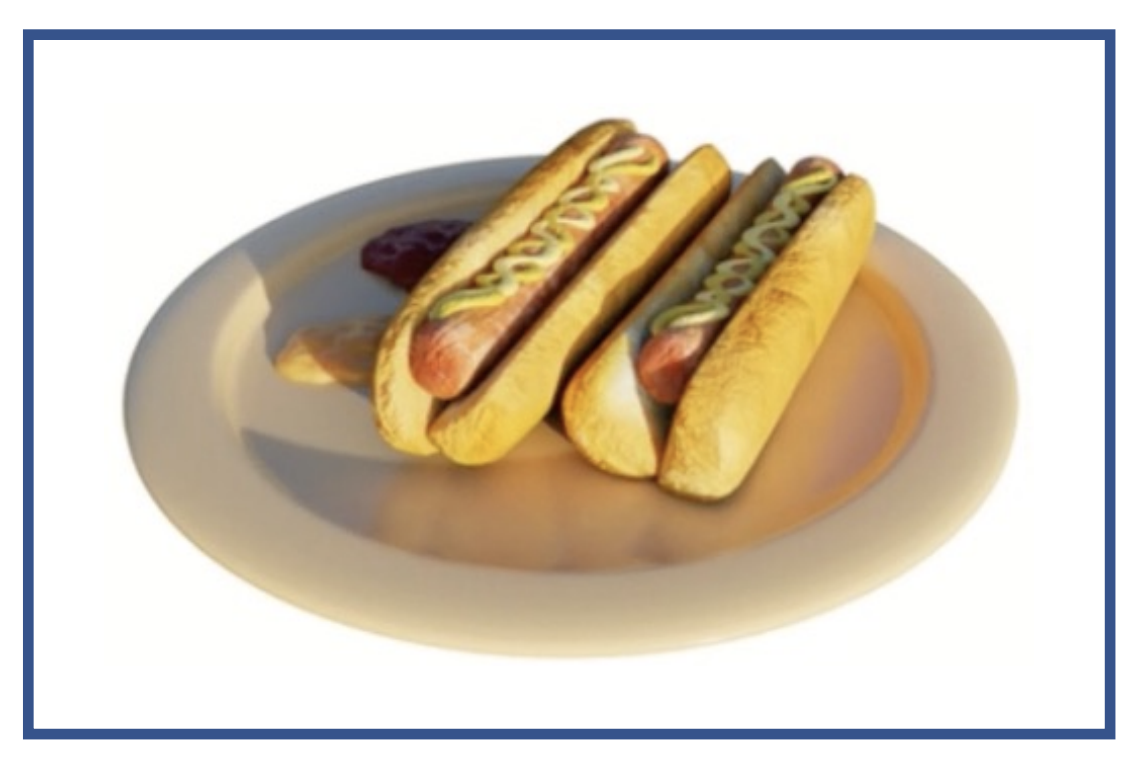
\includegraphics[width=\textwidth]{figures/model_6.png}
        \caption{The final output image after alpha blending (sorted by depth). }
        \label{fig:model_6}
    \end{subfigure}
    \hfill
    \caption{Overview of the rendering pipeline for the differentiable point-based radiance fields algorithm} 
    \label{fig:model_1to6}
\end{figure*}


The underlying model is represented by a point cloud in 3d space. Each point has a location parameter $P = (x, y, z)$ and a radiance parameter $H$. These parameters are learnt via stochastic gradient descent (Figure \ref{fig:model_1})

The rendering algorithm consists of two phases. In the first phase, the 3d point cloud is projected into 2d space and a view-dependent color is computed for each points. The mapping from 3d to 2d is accomplished with traditional camera math using $R, t, M$, with depth information also retained. The radiance parameter $H$ is the spherical harmonic parameters, which can be combined with $R, t, M$ to compute a view-dependent RGB color (Figures \ref{fig:model_2} and \ref{fig:model_3}).

In the second phase, the 2d points (each with an associated depth and color) are splat rendered into the final output image. This involves using a Gaussian kernel to represent the density ($\alpha$) parameter that each point has on each pixel, so that the the $\alpha$ value that a point has on a pixel is inversely proportional to the distance between the pixel and the point's 2d location. Then, each pixel's color is computed using traditional alpha blending, where we use each points color $c$, depth $d$ and radiance $\alpha$ (Figures \ref{fig:model_4}, \ref{fig:model_5}, \ref{fig:model_6}). Since the entire pipeline is differentiable, stochastic gradient descent is applied to learn the point cloud parameters $(x, y, z, H)$ for all the points.

One important aspect of this algorithm is the initialization of the point cloud. This is done using a rejection sampling technique. The training data is assumed to provide an object mask that describes what is the foreground (\ie the object to be rendered) and the background (\ie what we would like to ignore). Points $(x, y, z)$ are sampled uniformly from 3d space, and only kept if they are consistent with all the masks in the training data. That is, each point is projected into 2d space of each training image, and only kept if it falls into the foreground mask of all the training images.

\subsection{Mask Corruption Simulation}

The use of the object masks is an important component of the differentiable point-based radiance field algorithm. It is also a limitation. The masks provided in the Blender dataset \cite{mildenhall2020nerf} are perfect, but in a real world application a mask will not be perfect.

We propose the following simulation of a less-than-perfect mask. Set a parameter $x \in [0\%, 100\%]$ (\ie the ``corruption level''). For each image mask, apply a random affine transformation consisting of: a random rotation between $[-90x, 90x]$, translation between $[0, 0.5x*\text{(width or height)}]$, scaling between $[1-0.5x, 1+x]$, and shearing between $[0, 90x]$. Then, pass the imperfect masks as inputs to the original algorithm and measure the render quality.

\subsection{Proposed Solution to Imperfect Masks}

The corrupted masks changes the assumptions and provides a challenge to the existing algorithm. We propose the following solution to make differentiable point-based radiance fields more robust to imperfect masks.

First, relax the mask consistency constraint from a hard one to a soft constraint as suggested in \cite{zhang2022differentiable}. Originally, we only keep points which fall in all masks during the initialization step. Instead, we keep a point if it falls into at least $x\%$ of the masks. $x$ is a hyperparameter that must be chosen. 

Second, we add a pretraining step consisting of $7$ epochs of training only on the $P_\text{position}$ parameters of the model. Additionally, in the pretraining step, we use a new loss function.

$$L = ||f(I_\text{render}) - f(I_\text{ground-truth})||_2^2 +\lambda_\text{ridge} ||P_\text{position}||_2^2$$
$$f(I) = \tanh{(\max_\text{channel}(I) \cdot 5)}$$

\section{Analysis}

% Analyse your method: e.g., this is the place to report sensitivity w.r.t. a certain parameter, training curves, or ablation experiments with or without a loss that you try out.

The natural solution to the problem of imperfect masks is to relax the mask constraint. However, this is just part of the solution proposed. In this section, we motivate the pretraining step of the proposed solution.

First, observe that it is difficult to know, apriori, what hyperparameter to choose when relaxing the mask constraint. If too small of a number is chosen, \ie the mask constraint is relaxed too much, the initialized point cloud becomes highly inaccurate. For example, in Figure \ref{fig:outliers} observe that the initialized point cloud has degenerated into a ball around the object and there exists some outlier points which are not even attached to the main volume. This makes it challenging for the optimization.

\begin{figure}[h]
\centering
    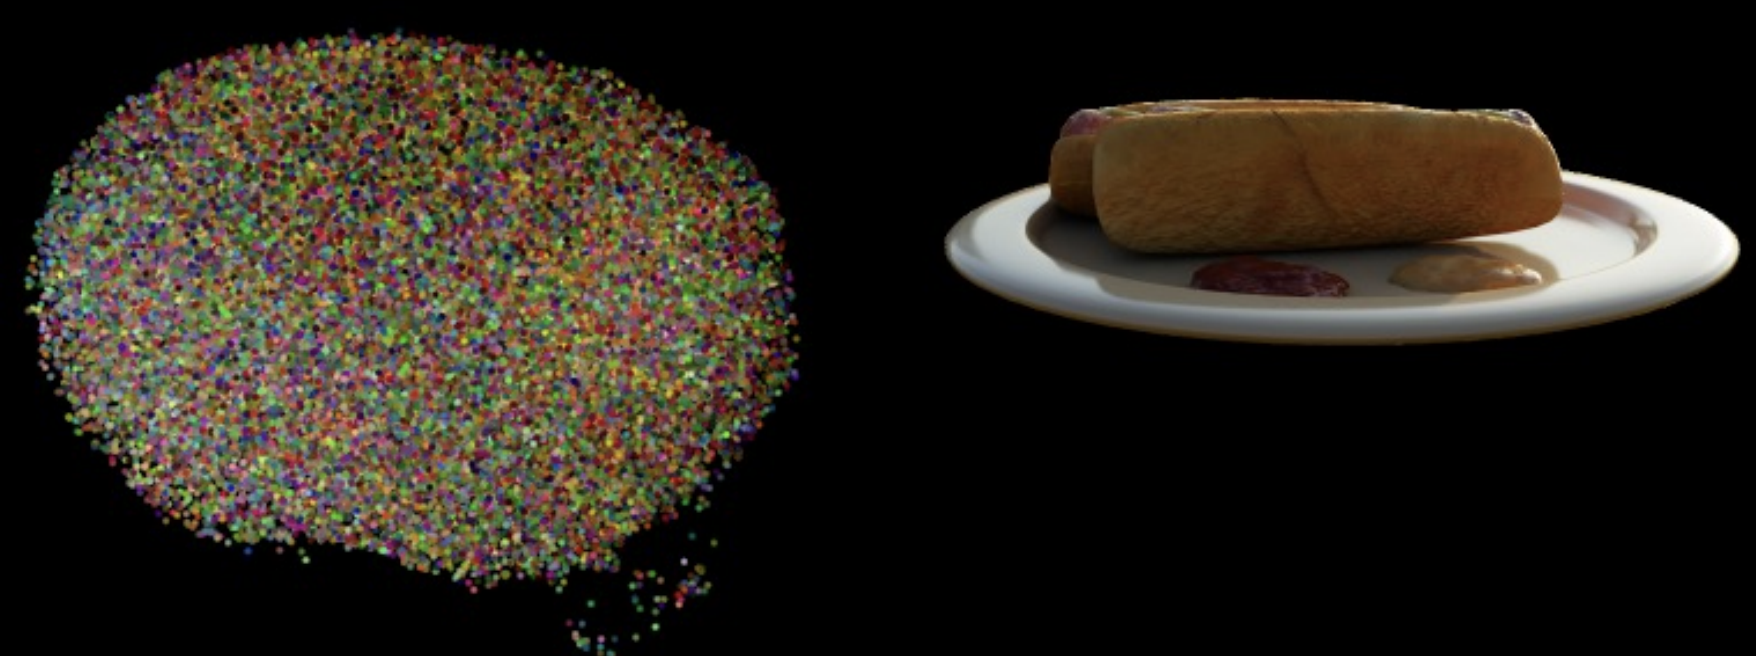
\includegraphics[width=0.90\linewidth]{figures/c12m70-init-outliers.png} 
    \caption{Corruption level 12\%, mask consistency threshold 70\%. The initial point cloud is on the left. The ground truth is on the right. Notice the outlier points in the bottom right of the  initial point cloud.}
\label{fig:outliers}
\end{figure}

Second, we observe that the dual optimization of radiance and position parameters makes it hard for a poorly initialized point cloud to converge to the right object volume positions. Figure \ref{fig:partialtraining} is an example of the model initialized with corrupted masks and relaxed mask constraints a few epochs into training. The initial point cloud is poorly initialized, such that many points are not where the object actually is. A few steps into training, the mass of points at the bottom (where there is no object in the ground truth) is being blacked out rather than their position being moved. Finally, in the final image there are artifacts below the object where no object should exist. From this, we hypothesize that the issue is that the dual optimization of position and color, when applied to a very inaccurate point cloud, will result in points being blacked out but not moved to their correct location, which leads to artifacts.

\begin{figure}[h]
\centering
    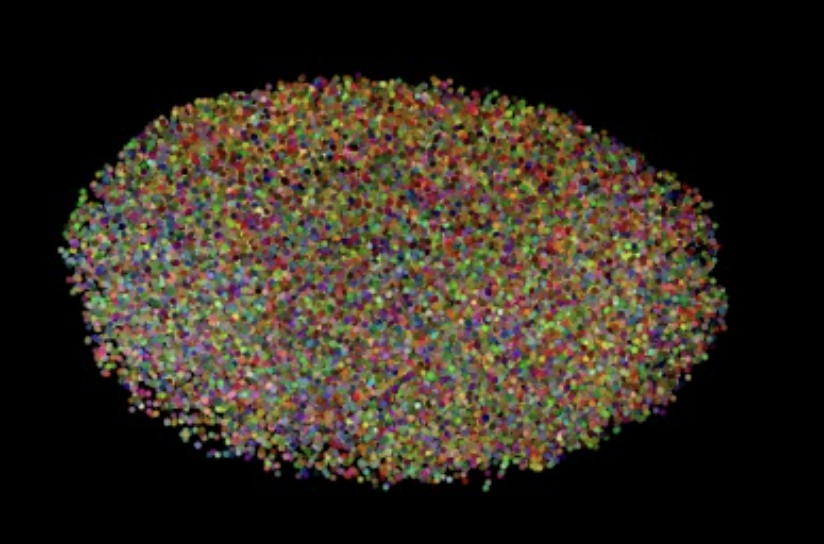
\includegraphics[width=0.45\linewidth]{figures/c12f80-0epochs.png}
    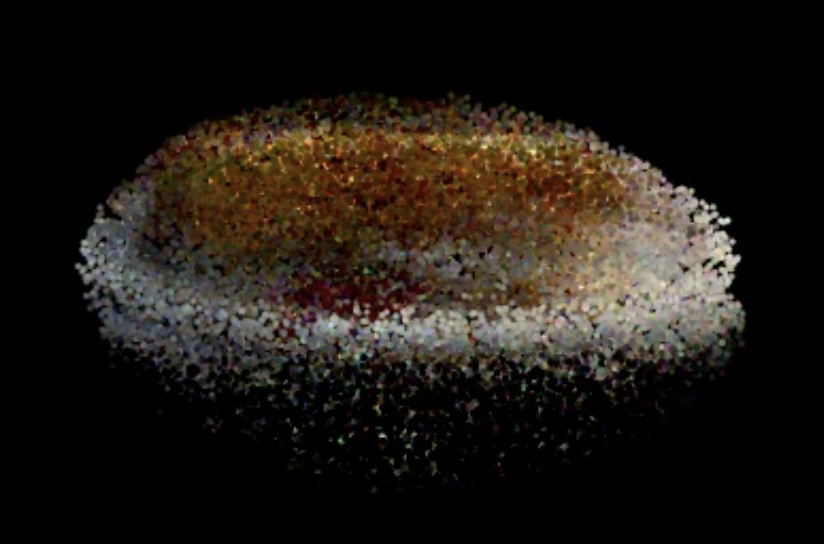
\includegraphics[width=0.45\linewidth]{figures/c12f80-5epochs.png} 
    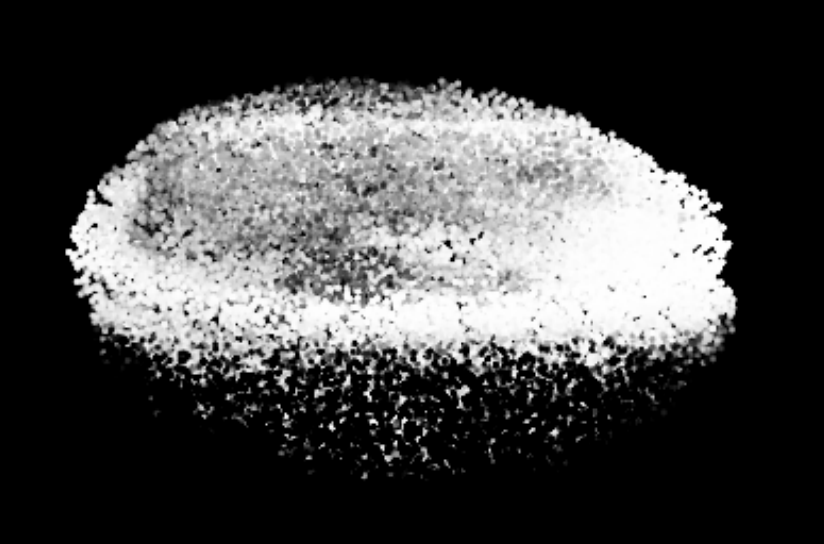
\includegraphics[width=0.45\linewidth]{figures/c12f80-5epochs-viz.png}
    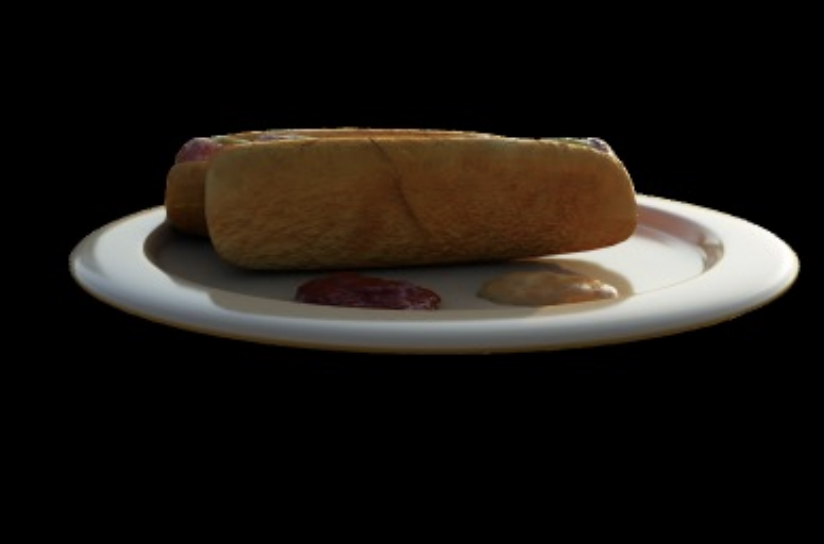
\includegraphics[width=0.45\linewidth]{figures/c12f80-gt-smal.png} 
    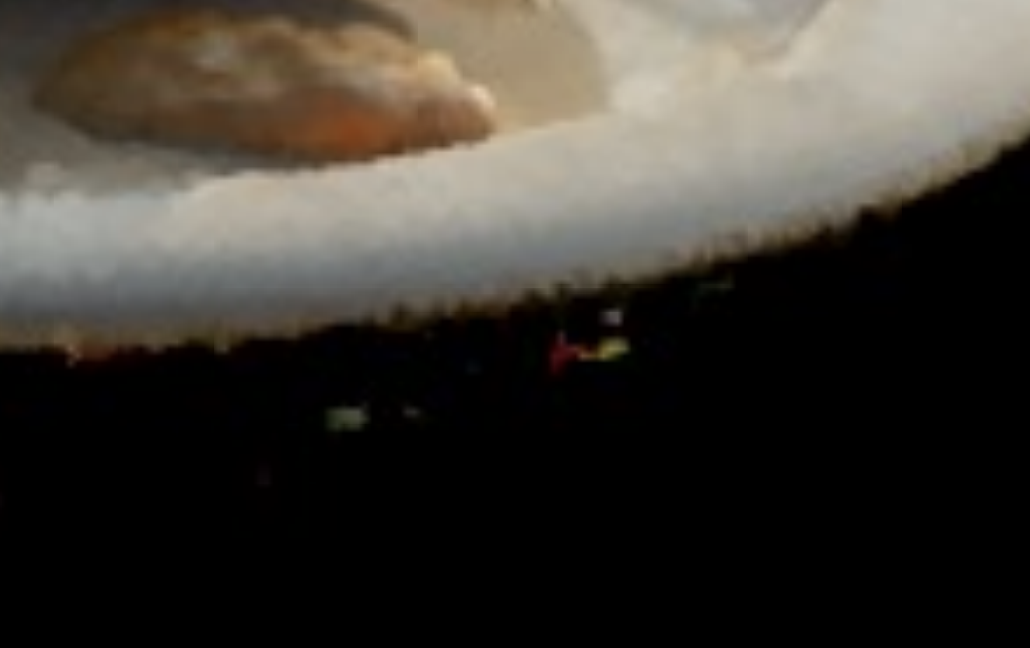
\includegraphics[width=0.45\linewidth]{figures/c12f80-artifacts.png} 
    \caption{Corruption level 12\%, mask consistency threshold 80\%, no pretraining step. 
    Initial point cloud (top left), after 5 epochs of training (top right and bottom left), ground truth (bottom right), artifacts in the final render (bottom center).}
\label{fig:partialtraining}
\end{figure}

This motivates the pretraining step of the solution. In this phase, we train only the position parameters to avoid the ``blacking-out'' issue described above. Because we only care about the position and not the color, we pass both the ground truth and rendered image into the function $f$ which essentially binarizes the pixels. Finally, to handle the fact that the initialized point cloud may have outliers and be very poorly initialized, we add a shrinkage term to the loss to bias point positions towards the center. The prior being that the object is likely centered. In this sense, we are leveraging a similar inductive bias as the regularization techniques used in \cite{jain2022zeroshot} and \cite{yang2023freenerf}.

\section{Results}

% Report and discuss qualitative and quantitative results here.

\subsection{Mask Corruption Experiment}

We apply the mask corruption detailed earlier for corruption percentages in 0\% to 20\%. Then, we run the original, unmodified algorithm. We find that as the corruption percentage increases, the model render quality declines significantly (Figure \ref{fig:corruptionexperiment}). Interestingly, the model size decreases at a steady linear-like rate with corruption percentage but the model render quality decreases at a slow rate until 8 percent where it then decreases much more rapidly. This may suggest that the original algorithm is robust to small imperfections in the training object masks, but beyond a certain threshold, the optimization struggles to recover the original quality.

\begin{figure}[h]
\centering
    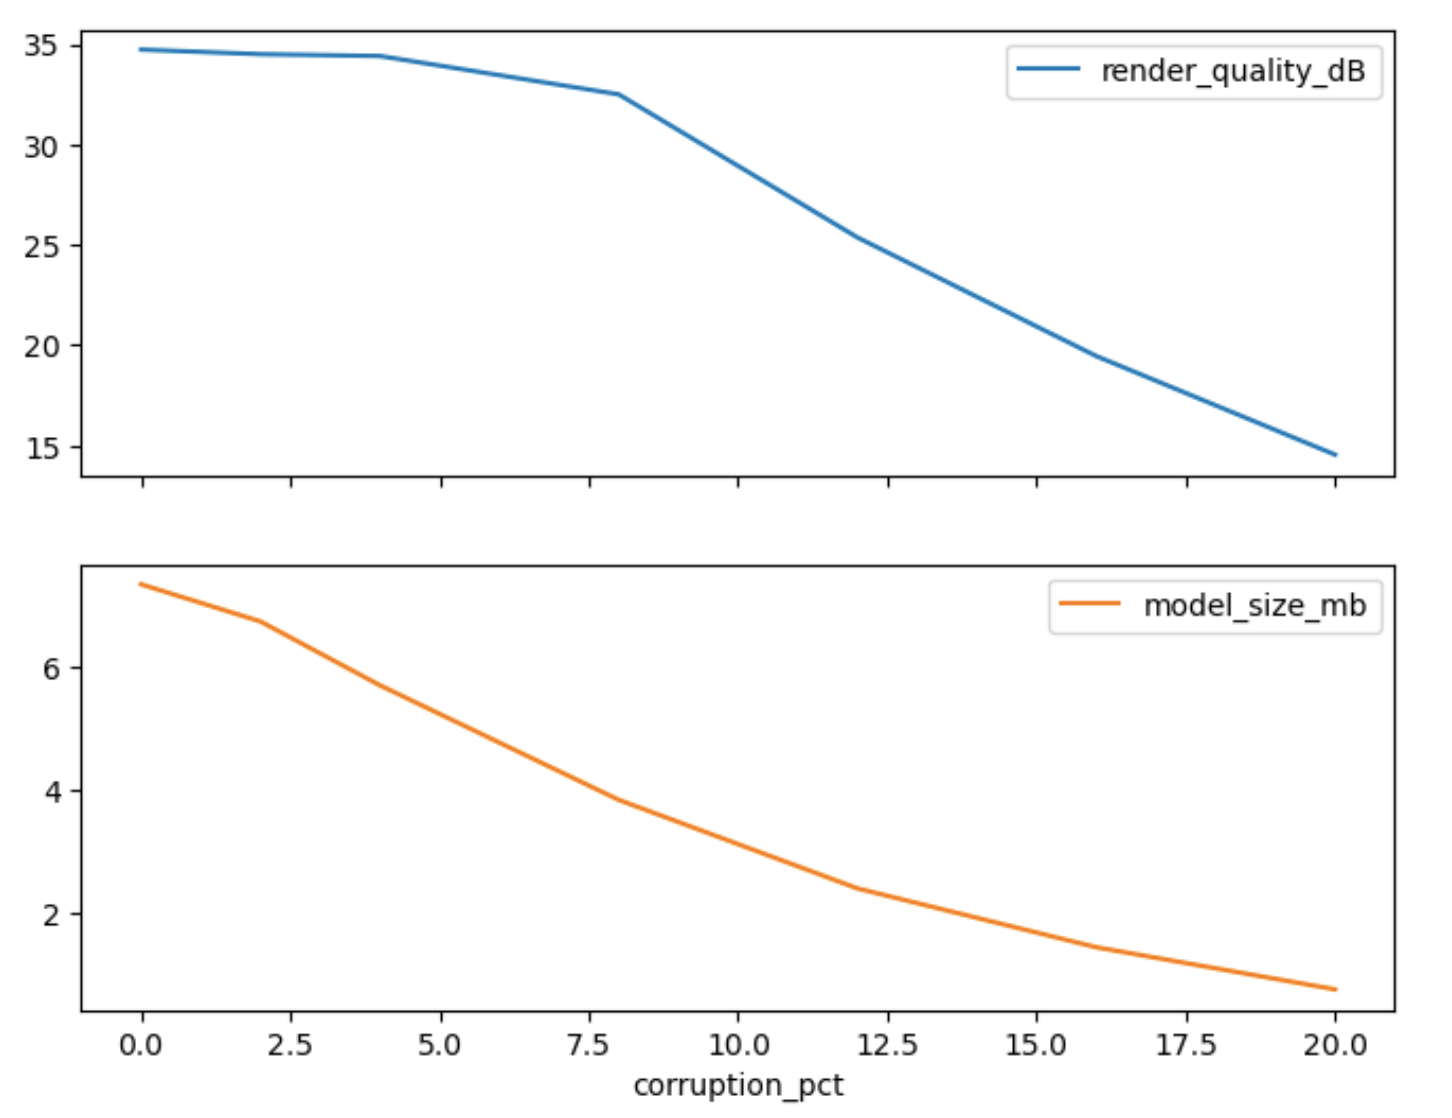
\includegraphics[width=0.9\linewidth]{figures/corruption-vs-quality-size.png}
    \caption{Varying the corruption level and running the unmodified algorithm. }
\label{fig:corruptionexperiment}
\end{figure}

Looking at the renders (Figure \ref{fig:corruptrenders}), we observe that as the corruption amount increases, the render becomes more and more sparse. By 12\% corruption level, the rendered output has sparse dot-like artifacts. Examining the initialized point cloud in Figure \ref{fig:maskoninit} (\ie the point cloud before any training is done), we see why: when the object mask corruption level increases, the volume in which the initialized point cloud is shrinks significantly and points are initialized in areas where the object is not present. This is in contrast to the initial point cloud generated from perfect masks: the object shape is almost perfectly captured before any training at all. So the imperfect masks presents two challenges. The first is that the masks are no longer multi-view consistent nor accurate so the hard rejection sampling mechanism is only able to initialize a small number of points in a small volume. Second, the initial point cloud from perfect masks is already close to the correct positions meaning there is not as much work for the optimization to do in terms of position, but for the imperfect masks the position optimization becomes very important.

\begin{figure}[h]
\centering
    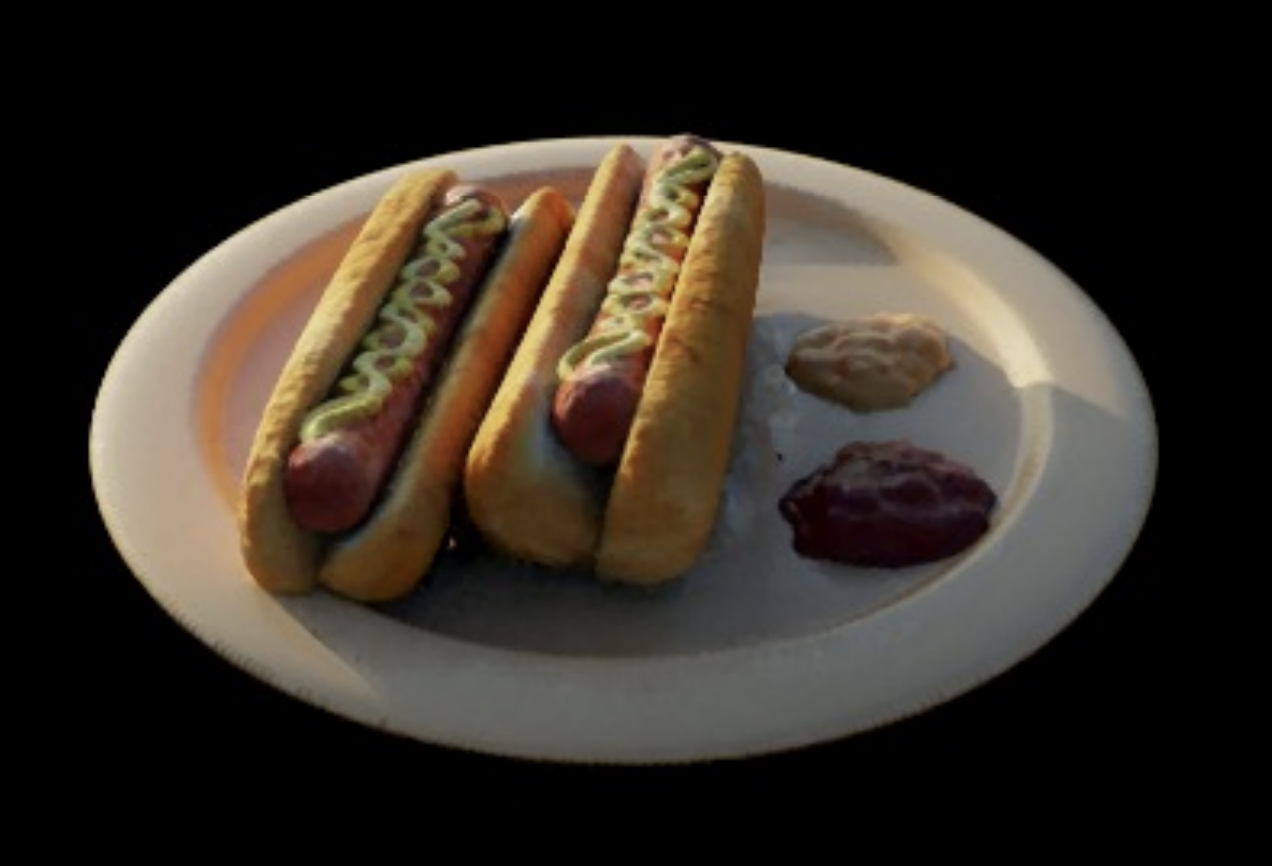
\includegraphics[width=0.45\linewidth]{figures/renderog.png}
    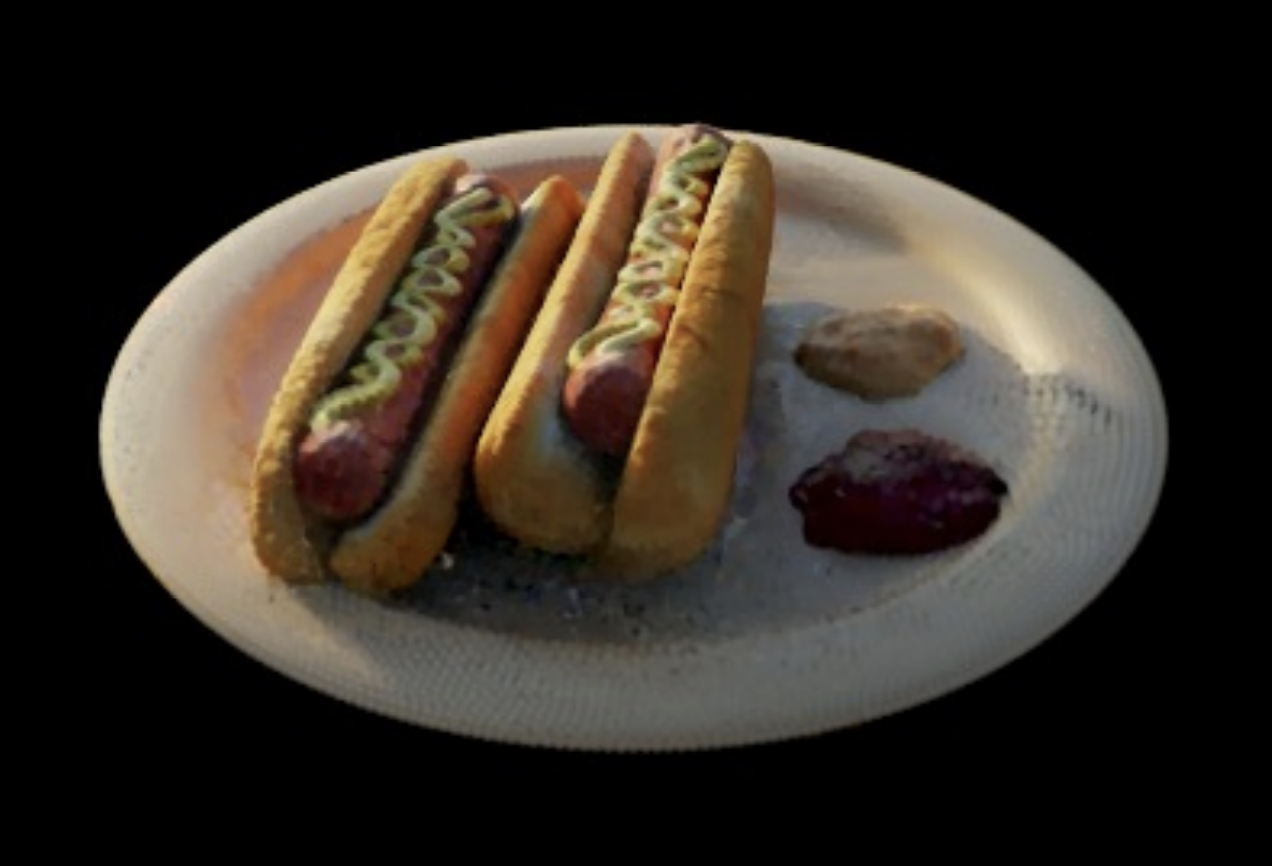
\includegraphics[width=0.45\linewidth]{figures/render8c.png} 
    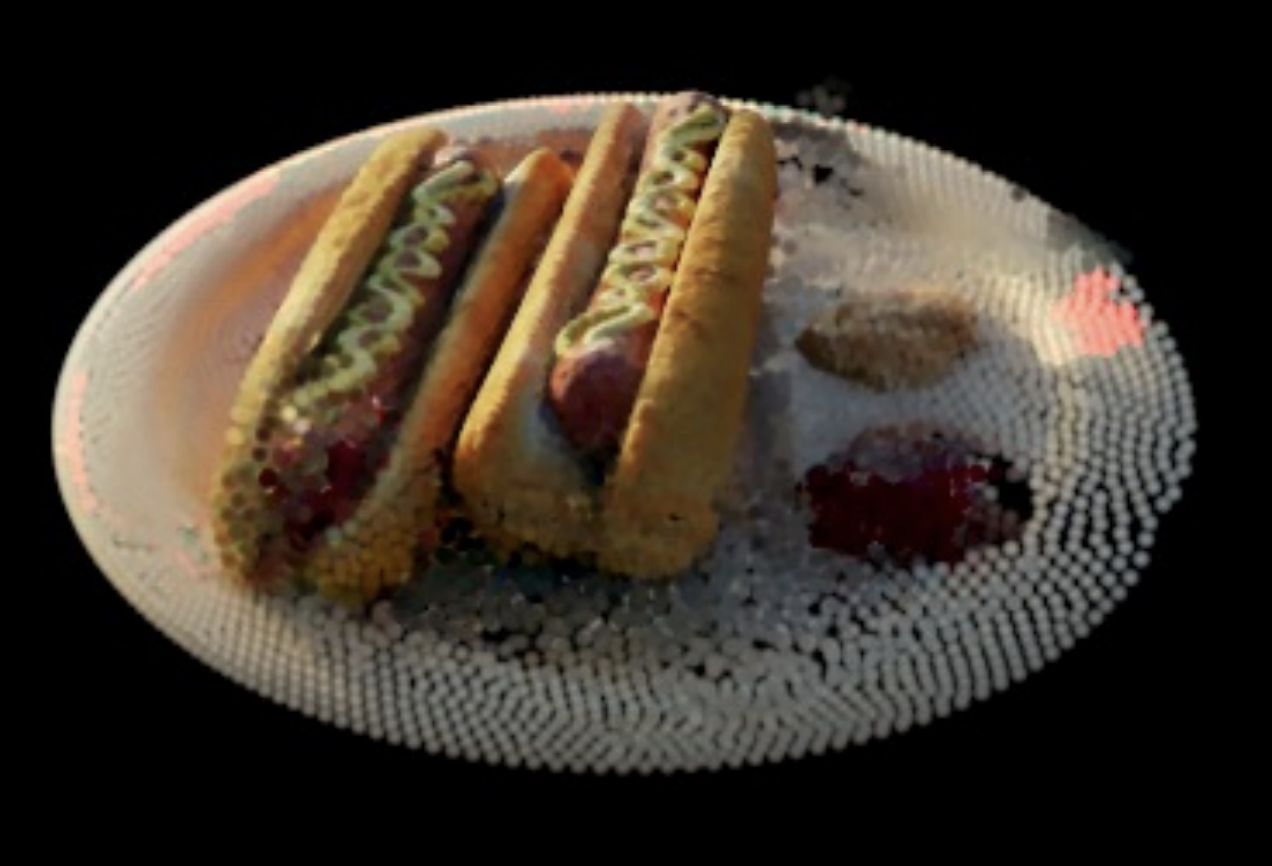
\includegraphics[width=0.45\linewidth]{figures/render12c.png} 
    \caption{Final renders of unmodified algorithm With corruption level of 0\% (top left), 8\% (top right), and 12\% (bottom). }
\label{fig:corruptrenders}
\end{figure}

\begin{figure}[h]
\centering
    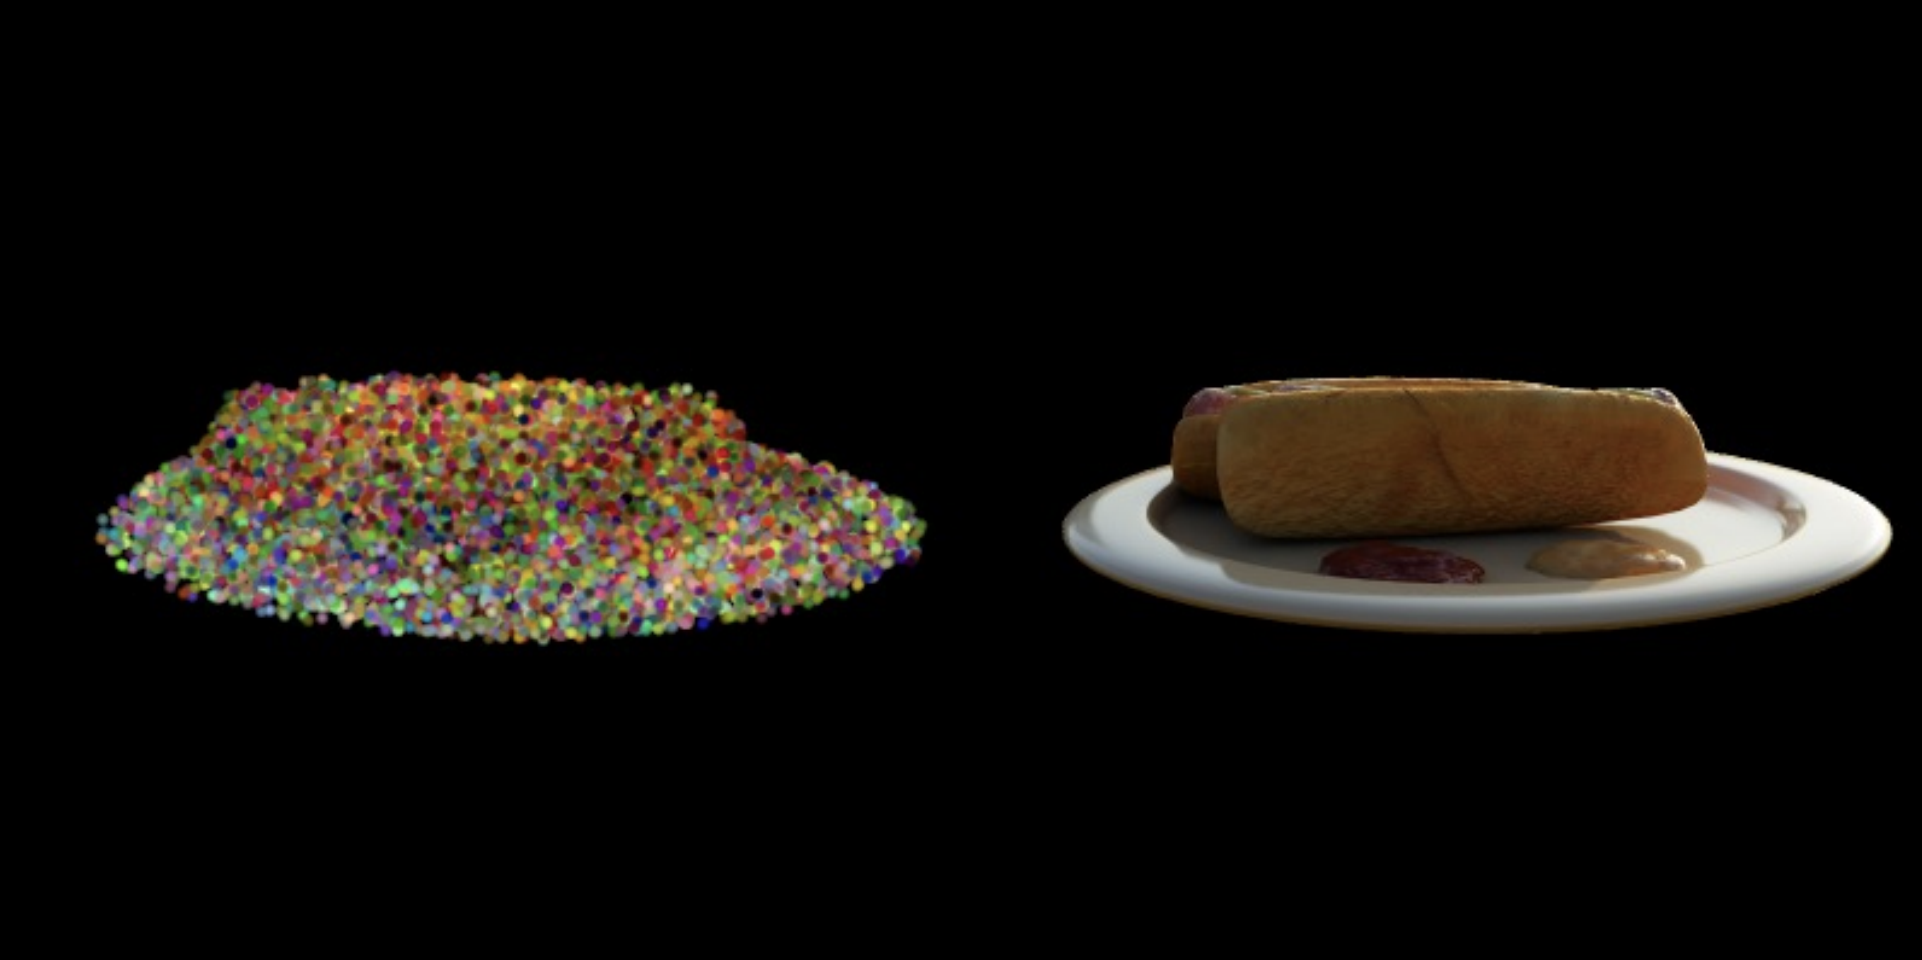
\includegraphics[width=0.45\linewidth]{figures/ogmask_1.png}
    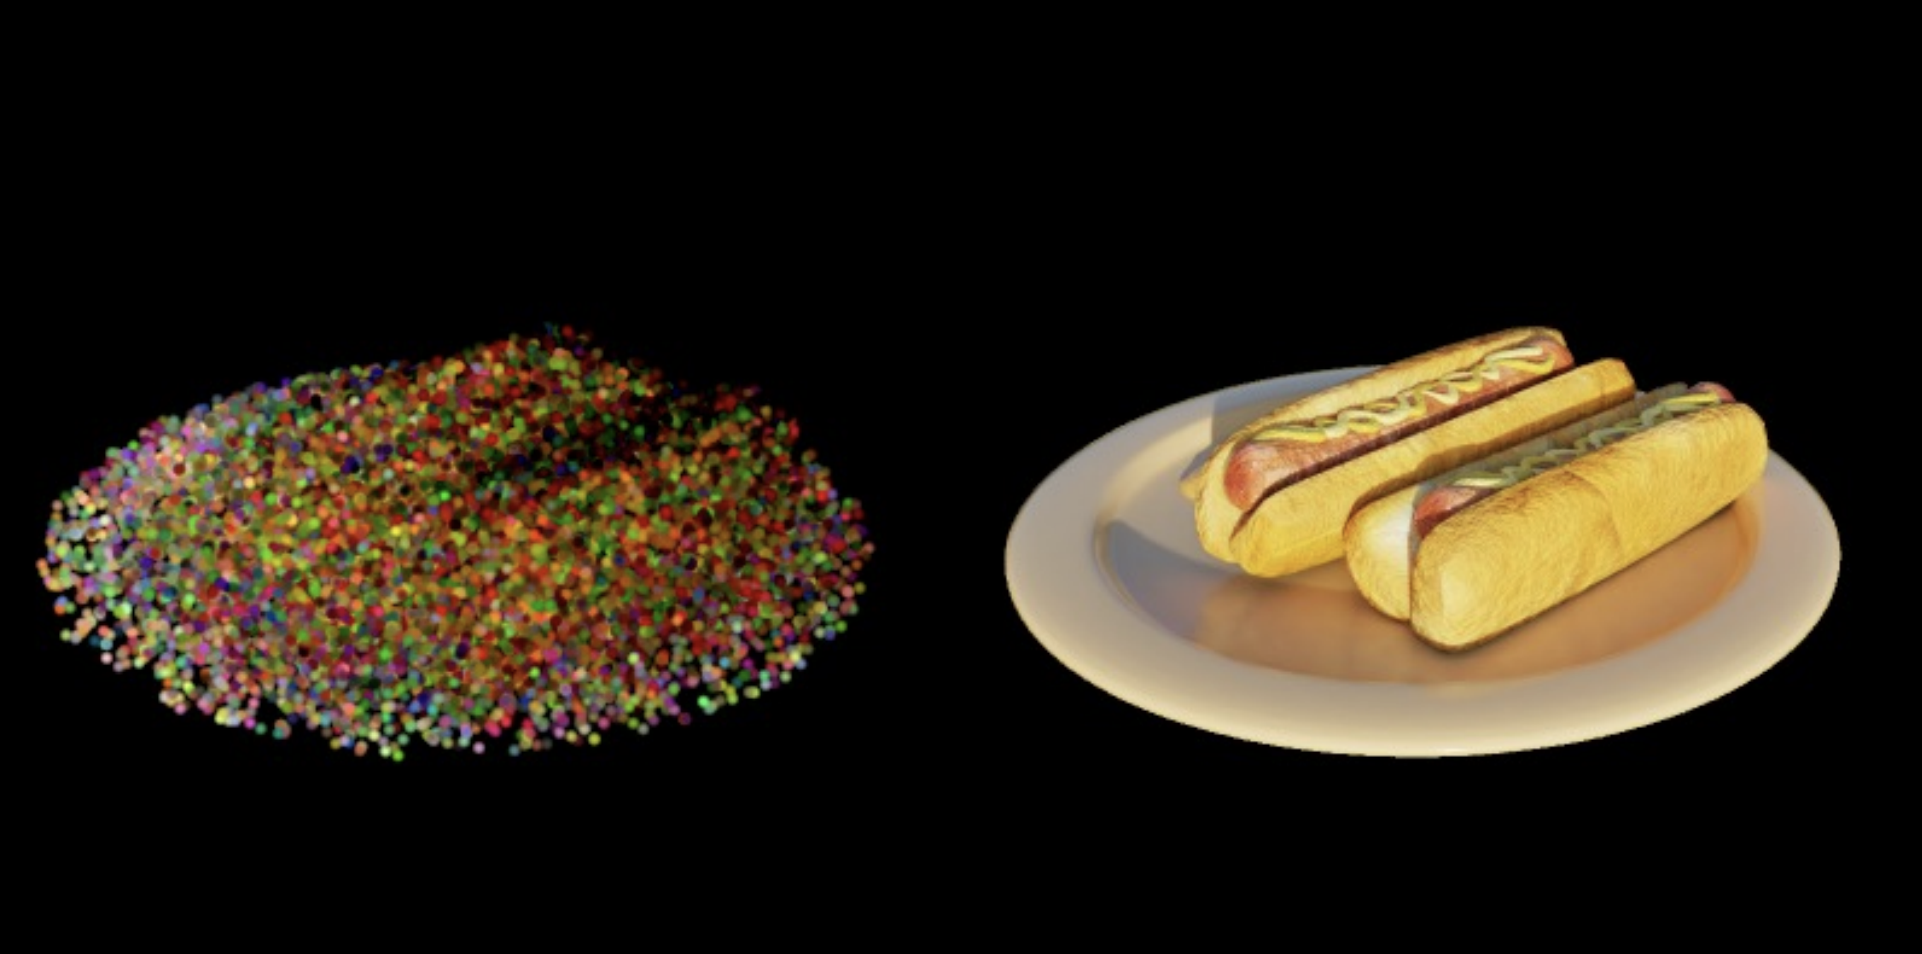
\includegraphics[width=0.45\linewidth]{figures/ogmask_2.png} 
    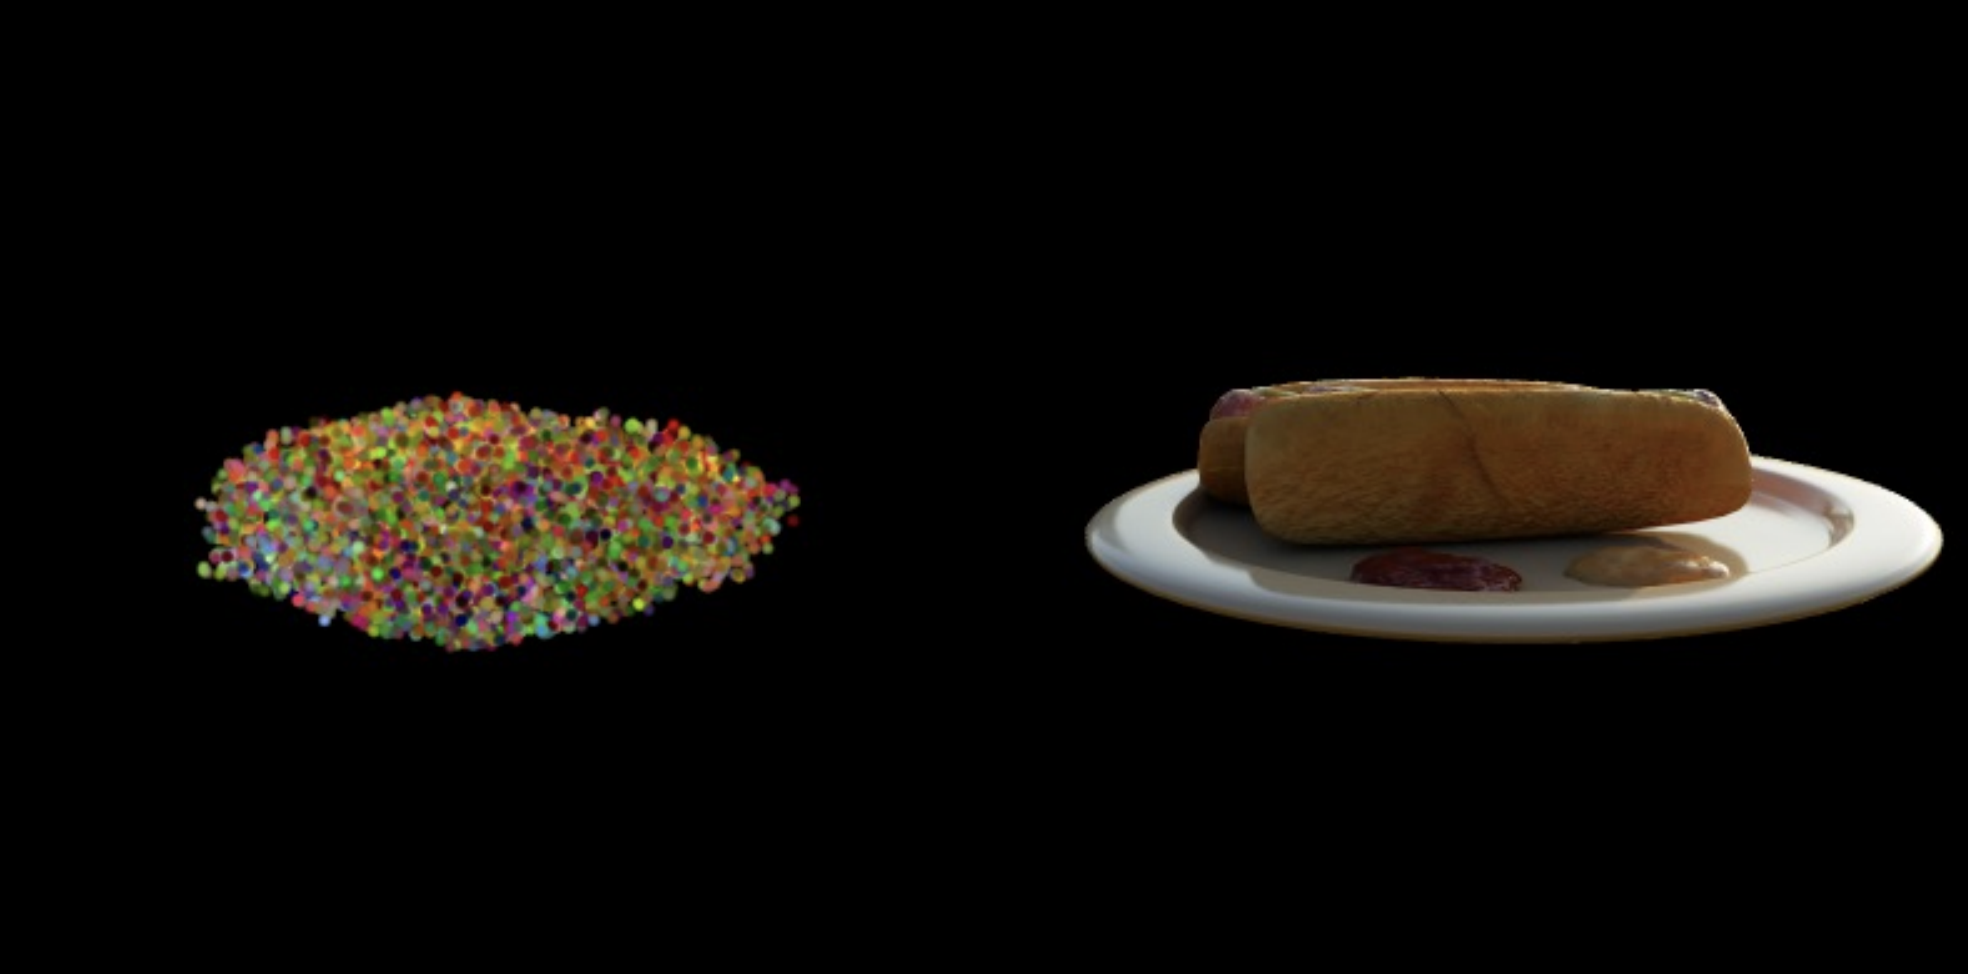
\includegraphics[width=0.45\linewidth]{figures/8pcorrupt-mask-1.png}
    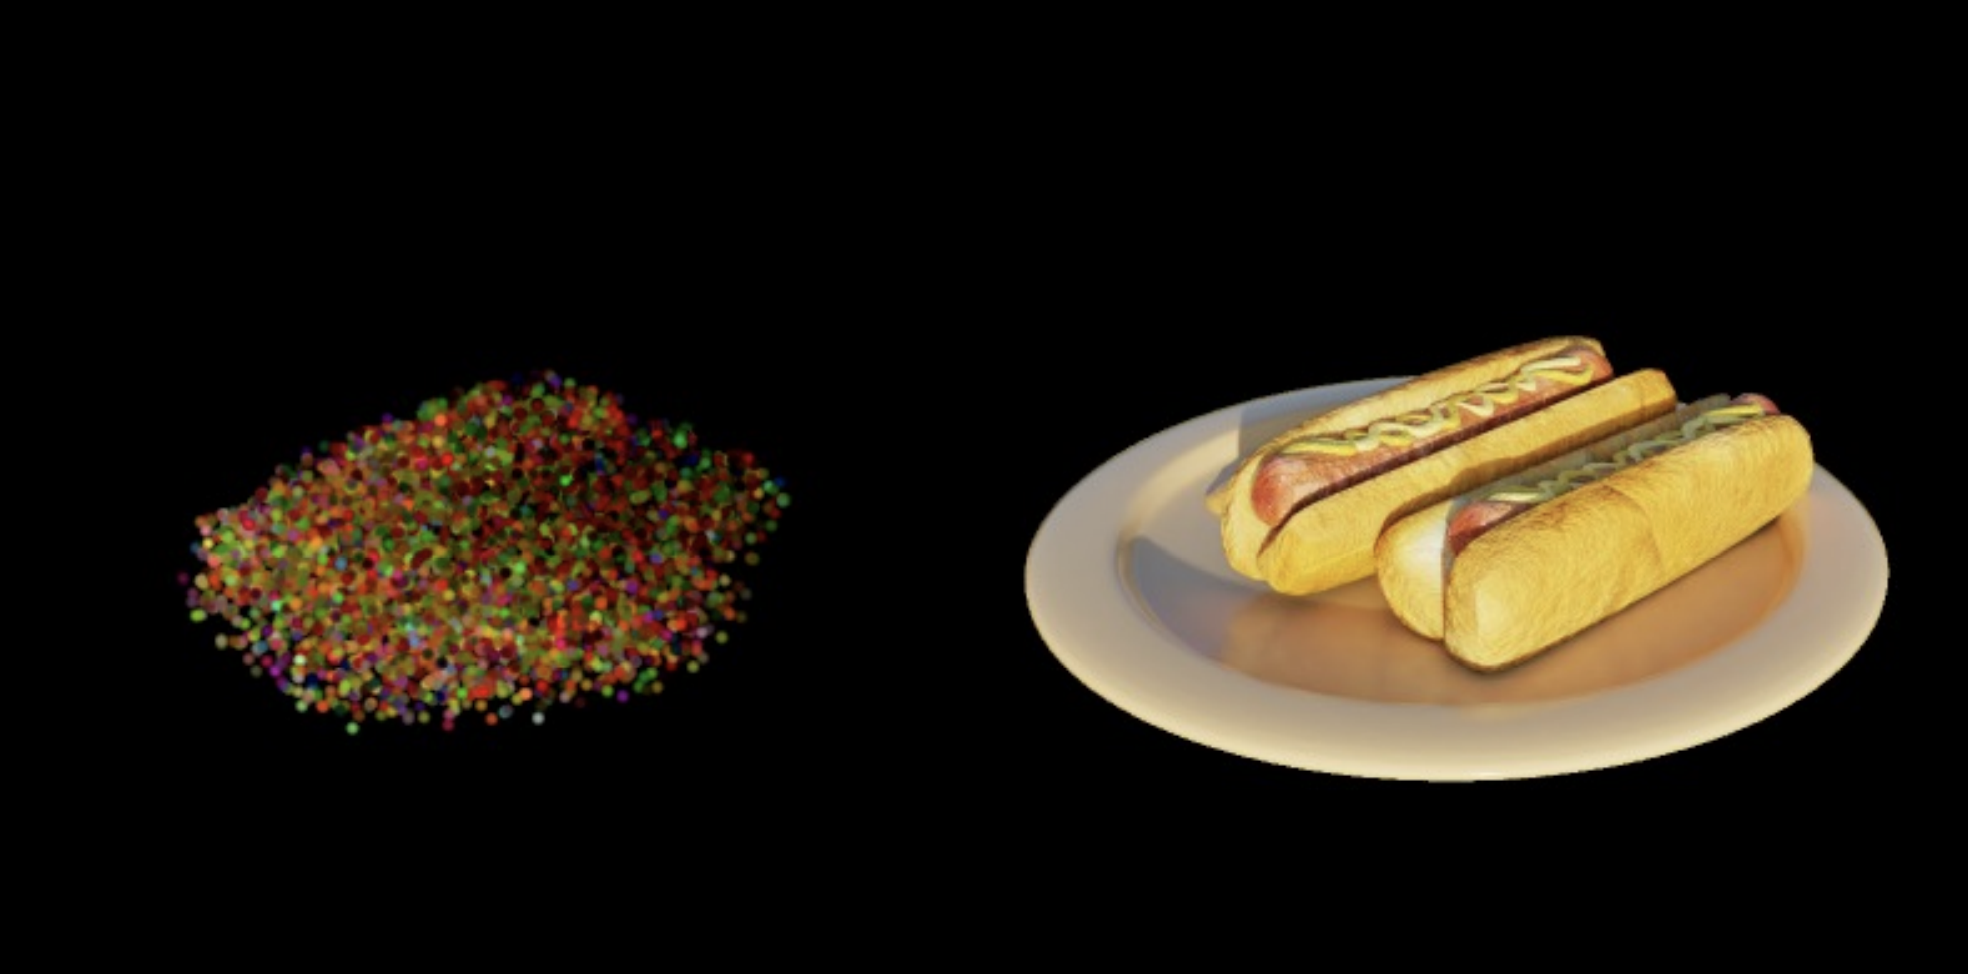
\includegraphics[width=0.45\linewidth]{figures/8pcorrupt-mask-2.png} 
    \caption{The inital point cloud with corruption level 0\% (top row) and 8\% (bottom row). }
\label{fig:maskoninit}
\end{figure}

\subsection{Evaluation of Proposed Solution}

We fix the corruption percentage at 12\% and investigate the efficacy of the first part of our proposed solution: relaxing the mask constraint from a hard one to a soft one. We run the algorithm and vary the mask consistency ratio from 100\% (\ie the original unmodified algorithm) to 70\% (\ie we keep an initial point if it falls in 70\% of the training masks). As the mask constraint is relaxed, the render quality improves dramatically to a level near the render quality of the original algorithm on perfect masks. However, this improvement only happens up to the 90\% consistency requirement level. Once the mask constraint is relaxed further (\ie decreased from 90\%) the render quality starts to decline significantly (Figure \ref{fig:constraintexperiment}). This observation is supported qualitatively. In Figure \ref{fig:corruptionwrelaxrender}, we see that relaxing the mask constraint is only helpful to a certain point, after which the number of artifacts grows noticeably.

\begin{figure}[h]
\centering
    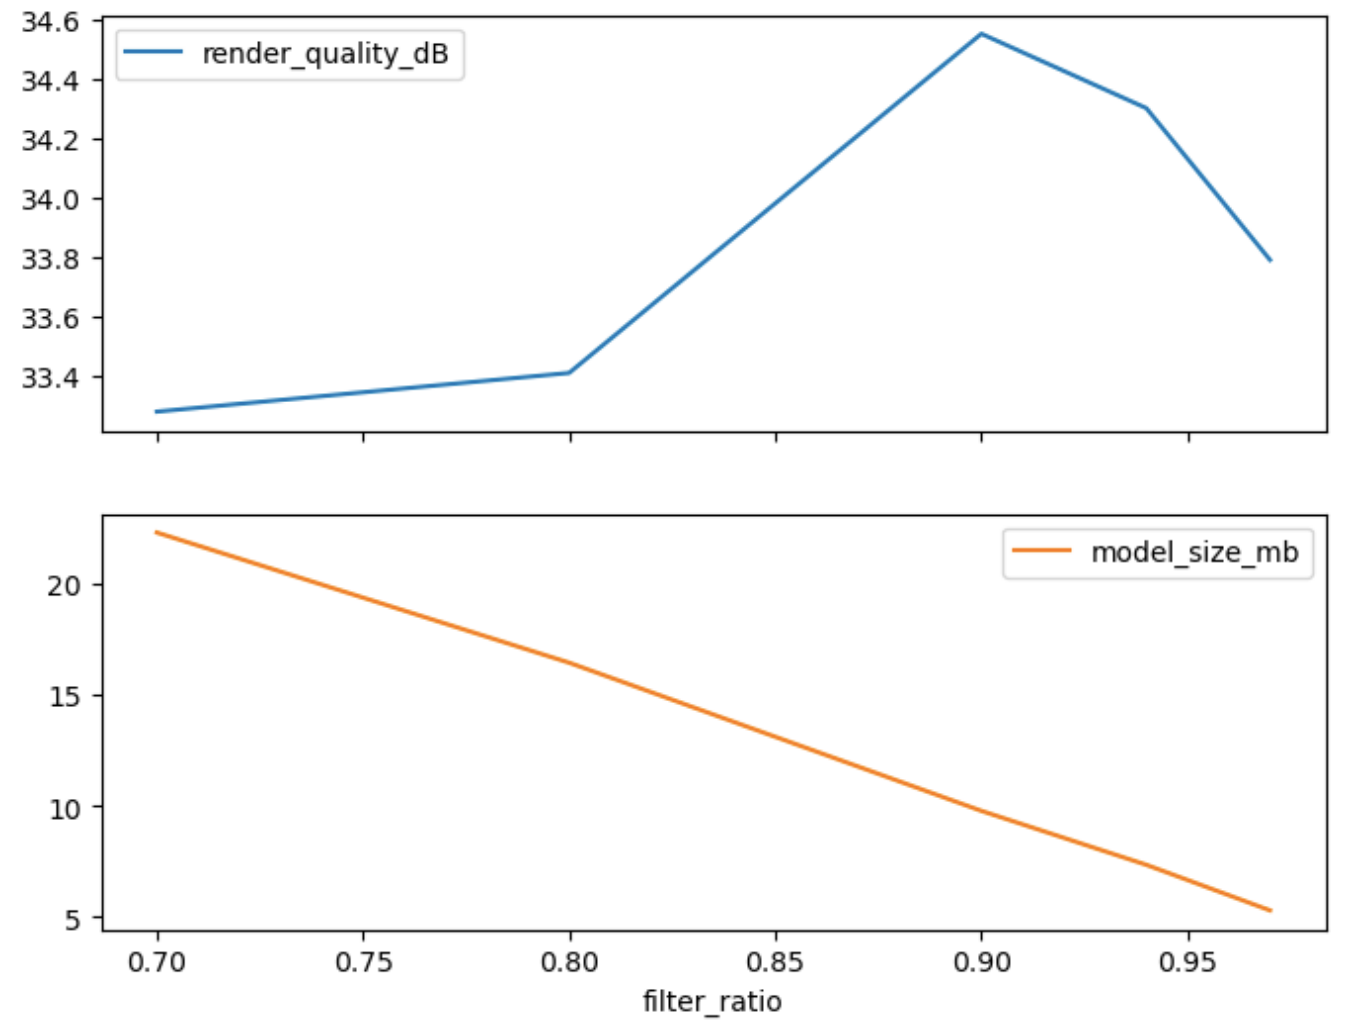
\includegraphics[width=0.9\linewidth]{figures/softconstraint-experiment.png}
    \caption{Experiment with fixed corruption level 12\% and varying mask consistency threshold. No pretraining step. }
\label{fig:constraintexperiment}
\end{figure}

\begin{figure}[h]
\centering
    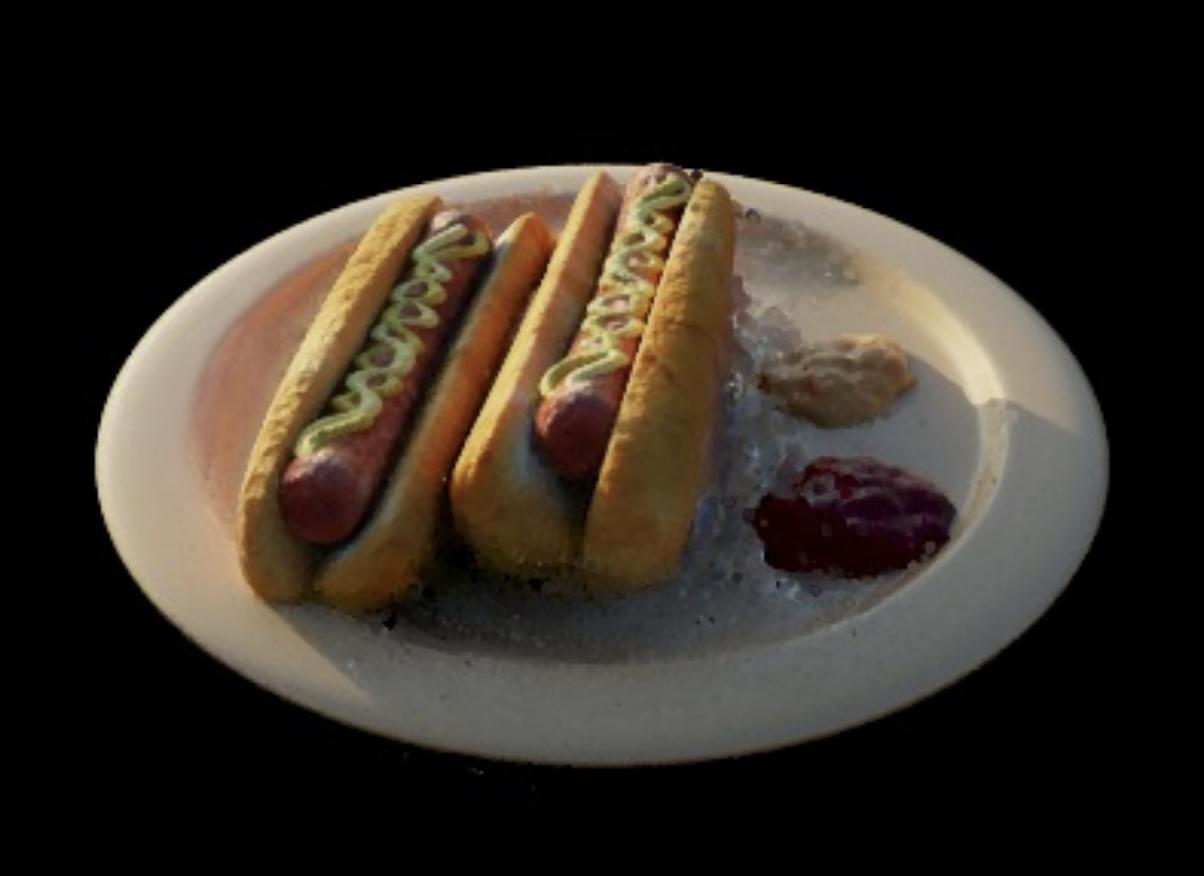
\includegraphics[width=0.45\linewidth]{figures/c12m70-r.png}
    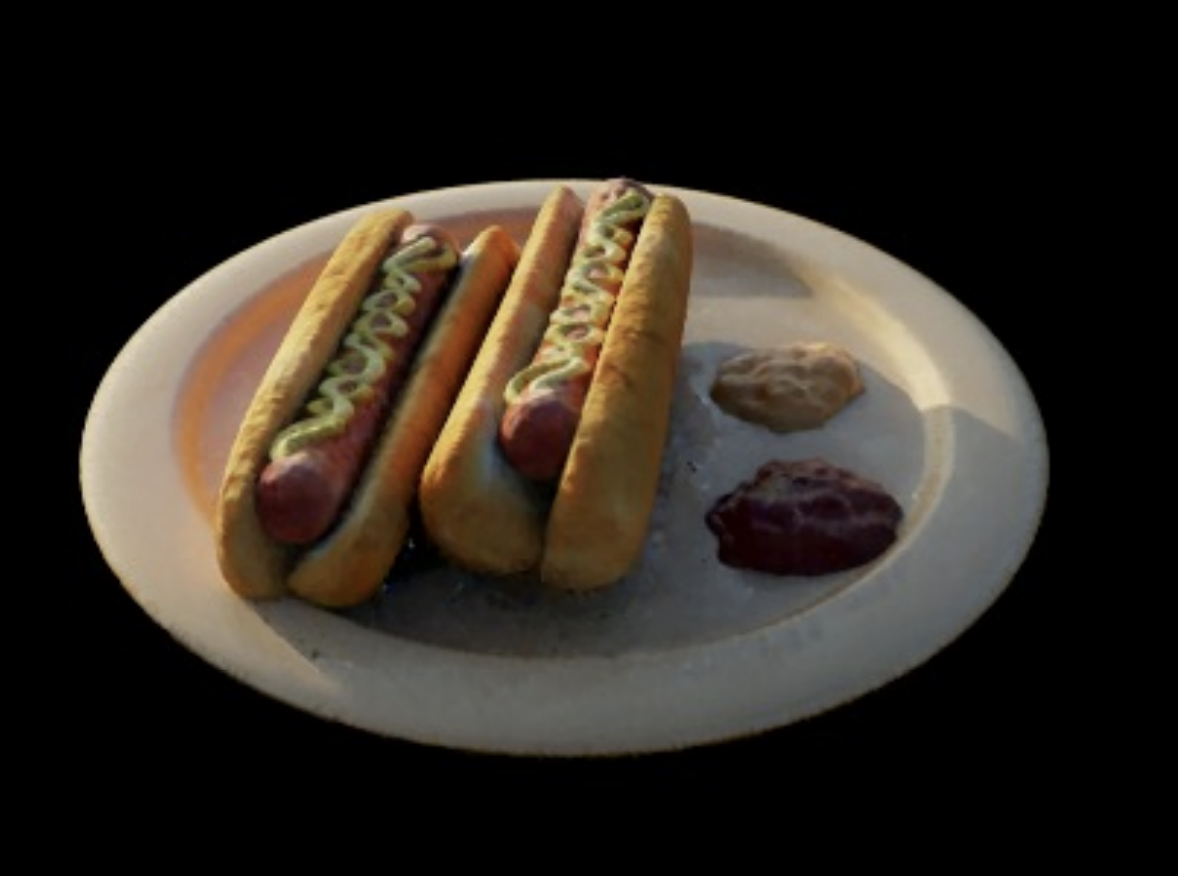
\includegraphics[width=0.45\linewidth]{figures/c12m90-r.png}
    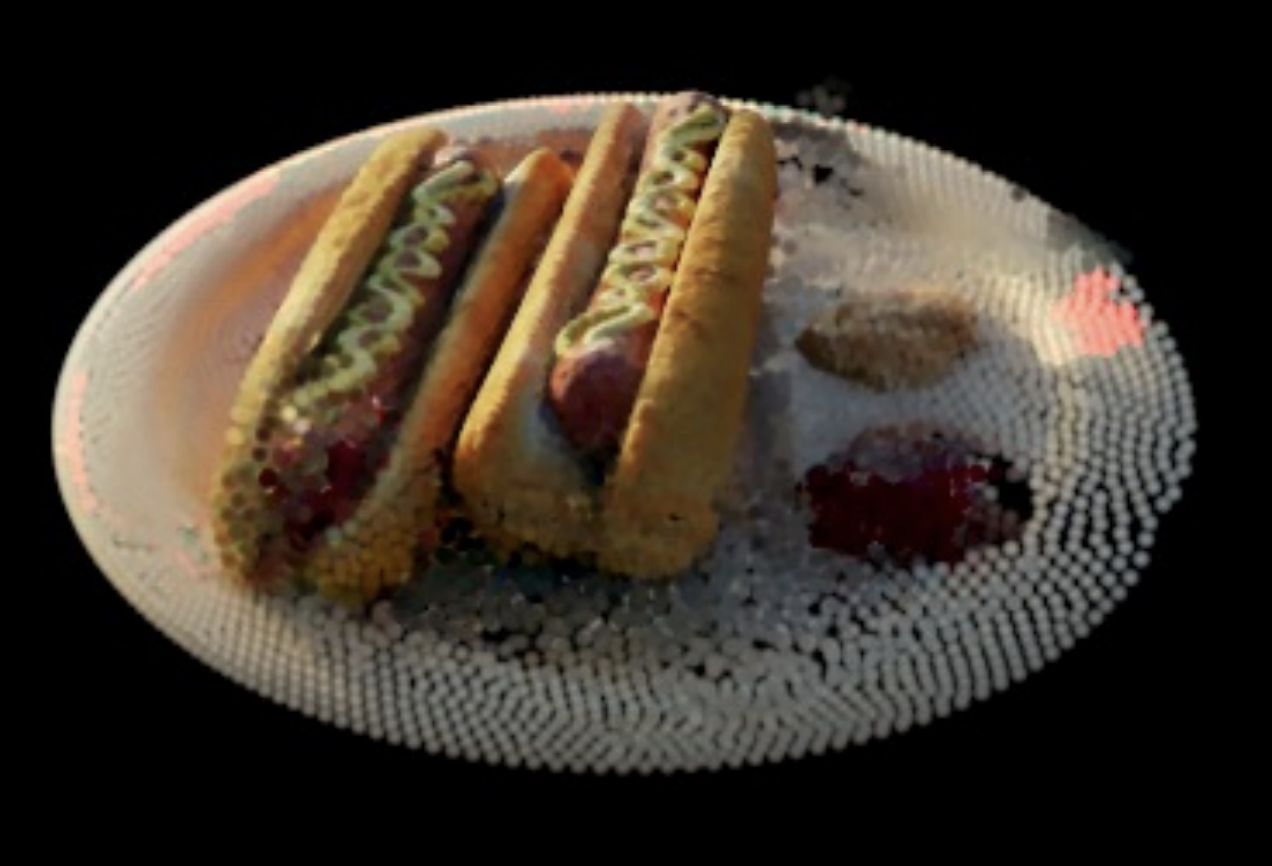
\includegraphics[width=0.45\linewidth]{figures/render12c.png} 
    \caption{ Final renders with fixed corruption level of 12\% and mask consistency threshold of 70\% (top left), 90\% (top right), 100\% (bottom). 
    }
    \label{fig:corruptionwrelaxrender}
\end{figure}

To understand further, we examine the initial point clouds before any training (Figure \ref{fig:corruptionwrelaxinit}). We see that as the mask constraint is relaxed the initial volume grows (also clear in Figure \ref{fig:constraintexperiment}). But the initial volume is highly inaccurate in both the high and low relaxation cases. It is more like expanding a spherical volume instead of actually matching the object volume. 

We hypothesize that relaxing the mask constraint introduces more points but in a not-well-informed manner (unlike with perfect masks). So with a small relaxation, the additional points are still close enough to the object volume that it is helpful in terms of final render quality. But as the relaxation grows, the additional points start being added at more and more irrelevant positions and this poses a major challenge to the optimization algorithm that eventually causes the net effect on render quality to be negative.

\begin{figure}[h]
\centering
    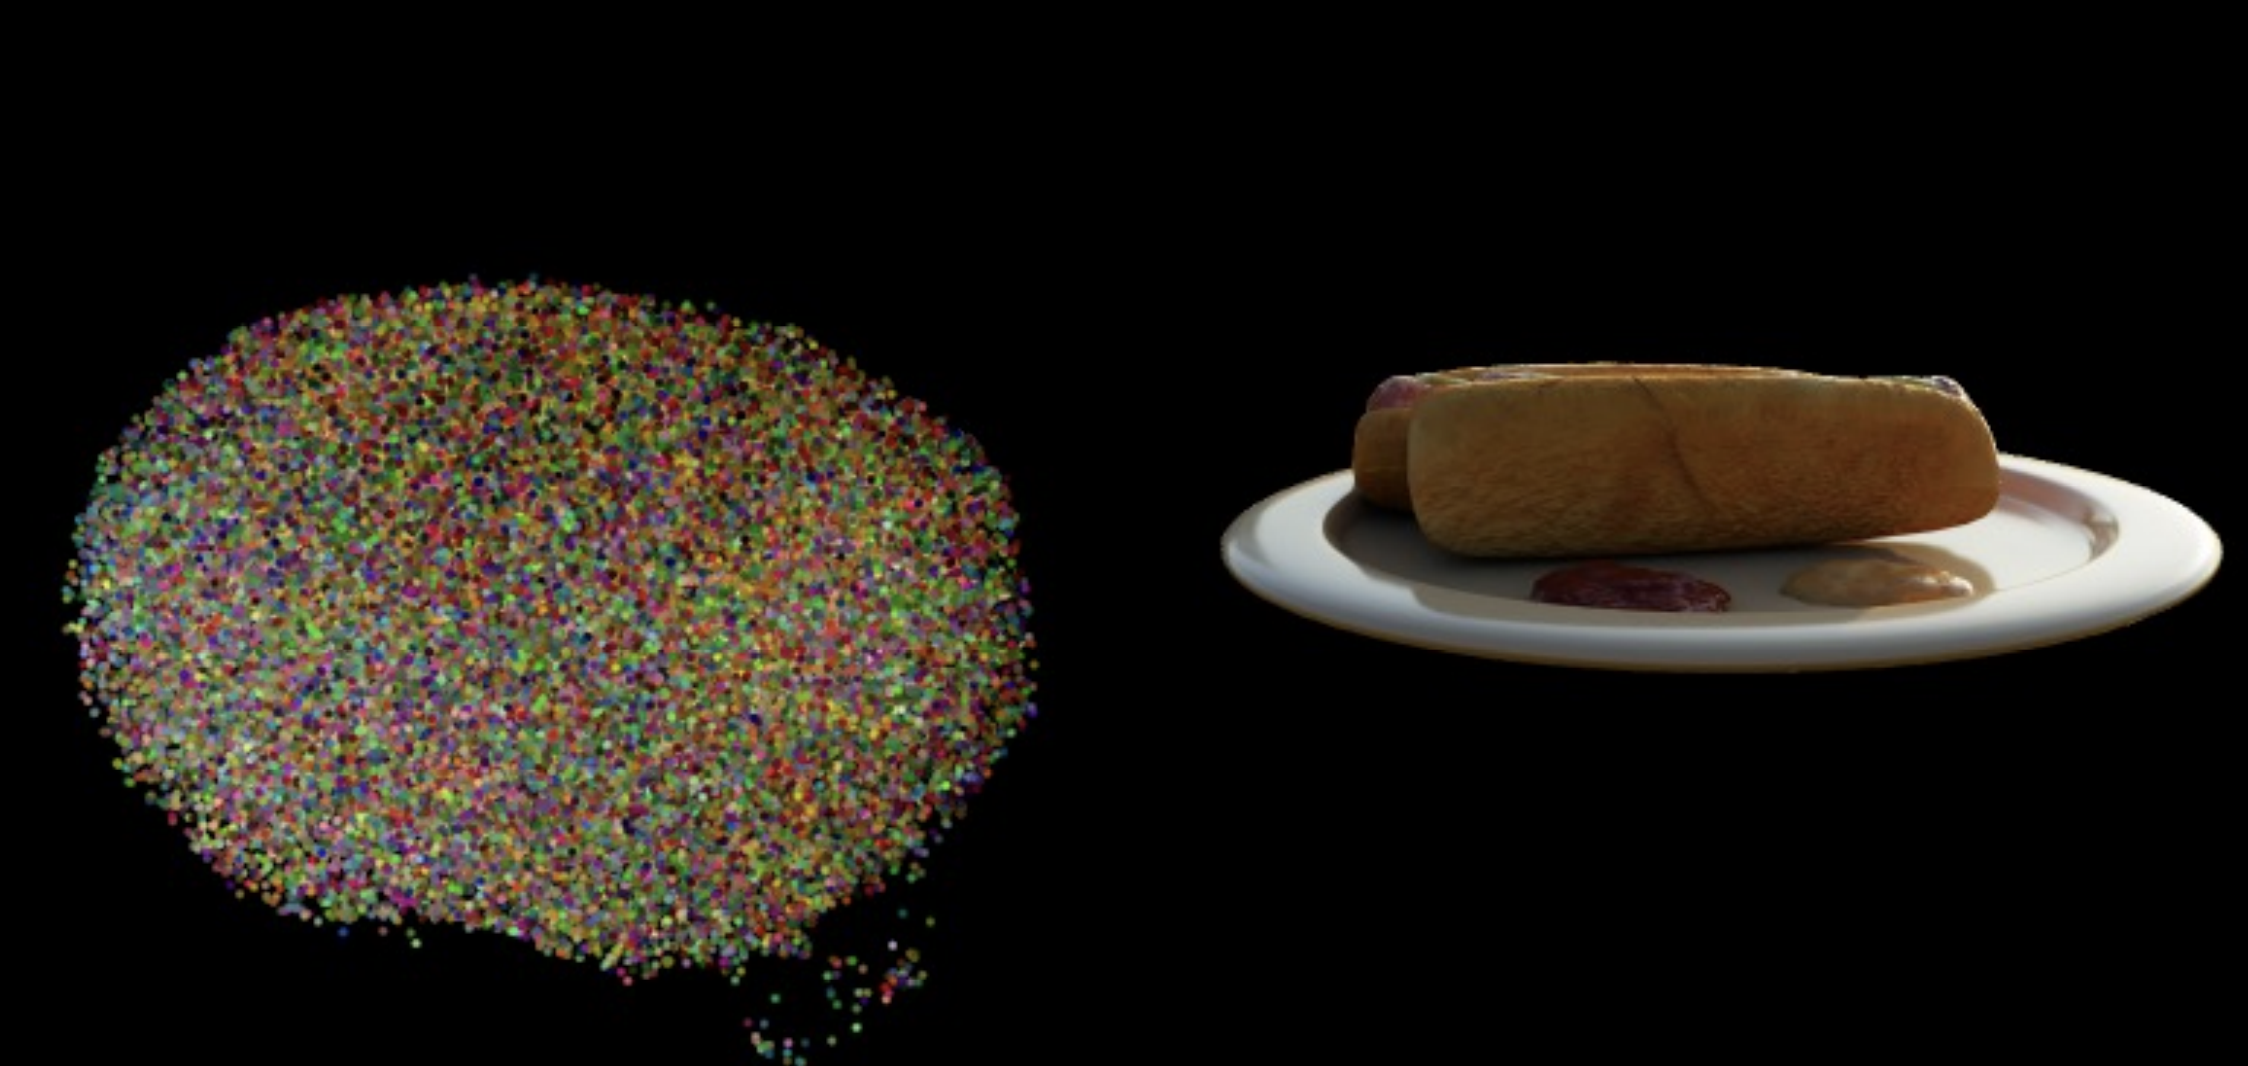
\includegraphics[width=0.9\linewidth]{figures/corrupt12mask70-init.png}
    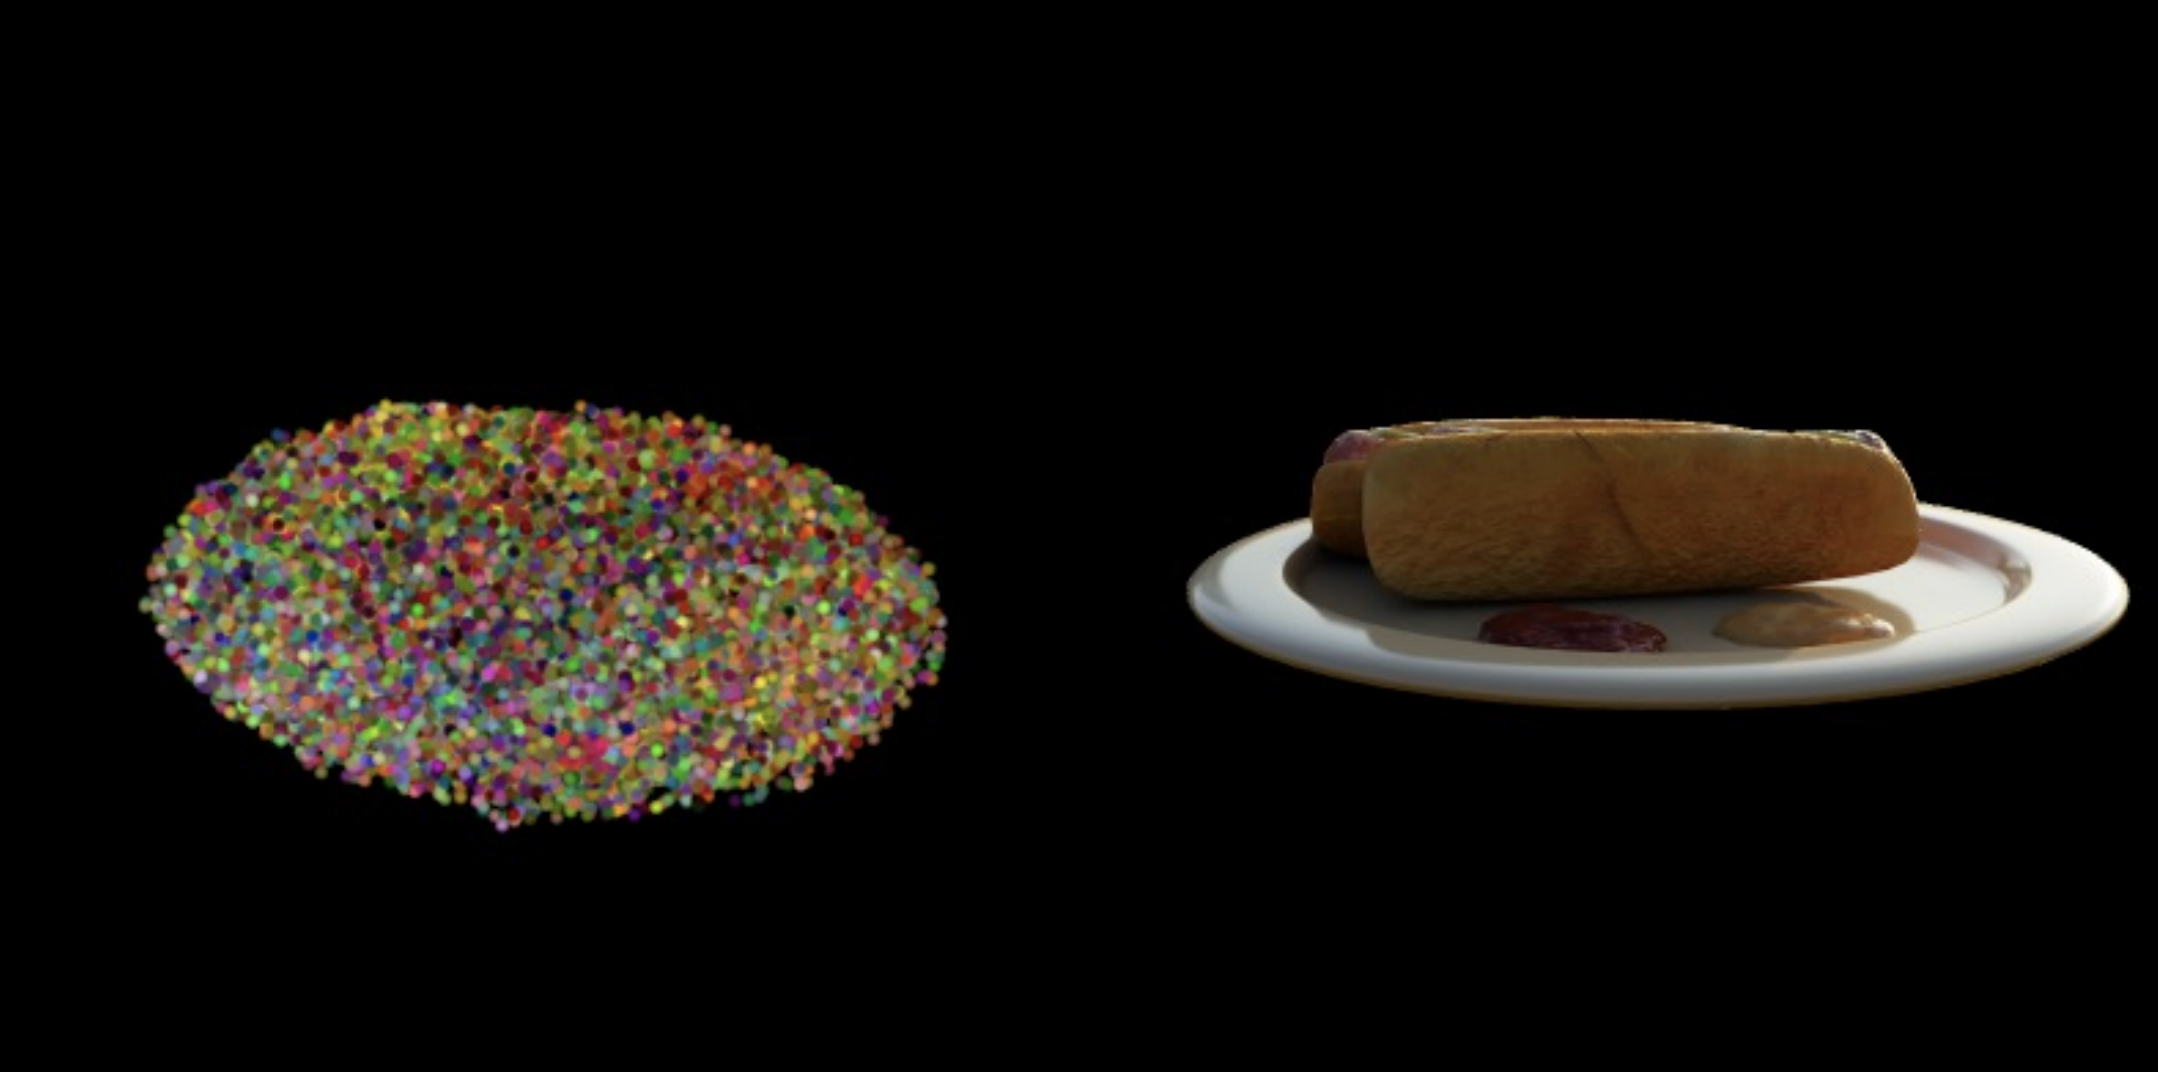
\includegraphics[width=0.9\linewidth]{figures/corrupt12mask90-init.png}
    \caption{ Initial point clouds with fixed corruption level of 12\% and mask consistency threshold of 70\% (left), 90\% (right).}
    \label{fig:corruptionwrelaxinit}
\end{figure}

Finally, we investigate the results of applying both stages of the proposed solution. Fixing the corruption percentage at 12\% and the mask relaxation constant at 80\%, we apply our pretraining step. Quantitatively, we improve the render quality (measured in PSNR) from 33.41 dB without the pretraining step to 34.12 with the pretraining. And we decrease the model size from 16.44 mb to 16.08. Qualitatively, we observe fewer artifacts (Figure \ref{fig:pretrainingqual}).

\begin{figure}[h]
\centering
    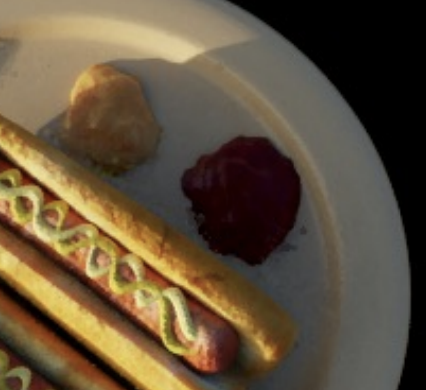
\includegraphics[width=0.45\linewidth]{figures/npre-1.png}
    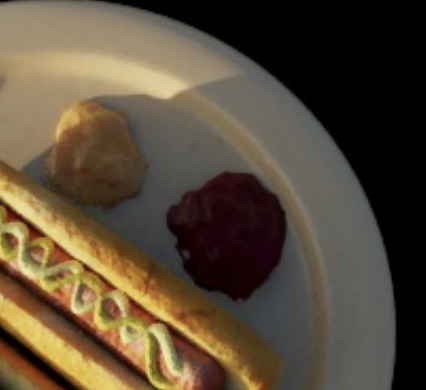
\includegraphics[width=0.45\linewidth]{figures/ypre-1.png}
    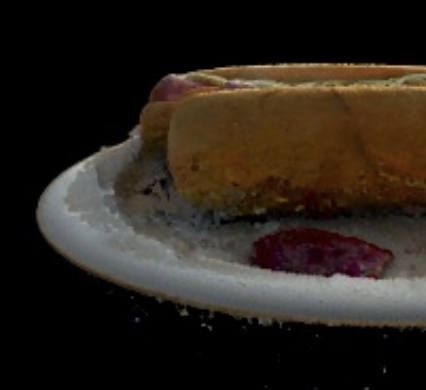
\includegraphics[width=0.45\linewidth]{figures/npre-2.png}
    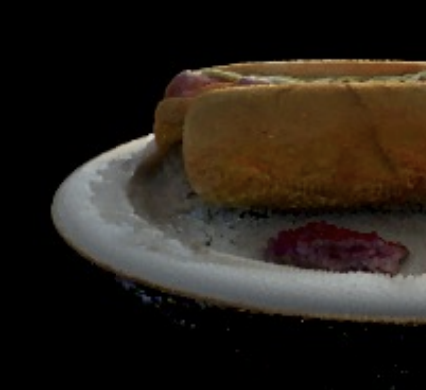
\includegraphics[width=0.45\linewidth]{figures/ypre-2.png}
    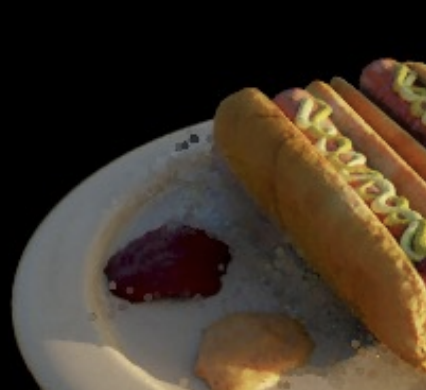
\includegraphics[width=0.45\linewidth]{figures/npre-3.png}
    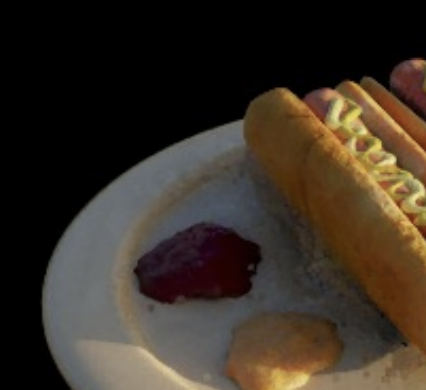
\includegraphics[width=0.45\linewidth]{figures/ypre-3.png}
    \caption{ Fixed 12\% corruption level and 80\% mask consistency threshold. Final renders with no pretraining step (left column) and with pretraining step (right column). }
\label{fig:pretrainingqual}
\end{figure}

To understand further how the pretraining step is helping, we examine the point cloud after initialization and after the pretraining step (Figure \ref{fig:pretrainingviz}). The initial point cloud occupies a volume that covers the real object volume but is highly inaccurate. After the pretraining step, we observe that the volume has shrunk significantly and begun to form sharper edges around the object volume, somewhat resembling the initial point cloud with perfect masks. We hypothesize the better shape of the initial point cloud after the pretraining step is responsible for the gains in render quality observed above.

\begin{figure}[h]
\centering
    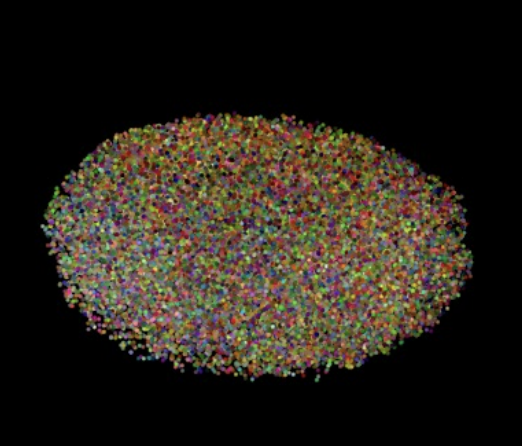
\includegraphics[width=0.45\linewidth]{figures/c12f80-b4pretrain.png}
    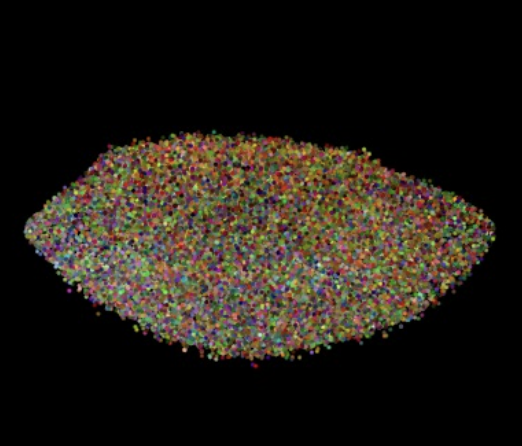
\includegraphics[width=0.45\linewidth]{figures/c12f80-afterpretrain.png}
    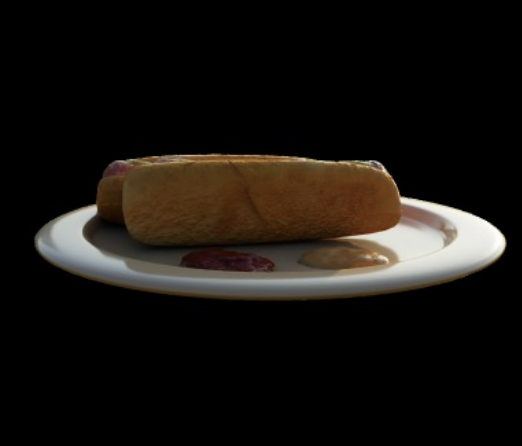
\includegraphics[width=0.45\linewidth]{figures/c12f80-gt.png}
    \caption{Fixed 12\% corruption level and 80\% mask consistency threshold. Point cloud at initialization (top left), after pretraining step (top right). Ground truth image (bottom).}
\label{fig:pretrainingviz}
\end{figure}

\section{Conclusion}

%discuss limitations of the approach and conclude your findings, keep this short

In this work, we explore the differentiable point-based radiance fields algorithm in a modified setting: that of imperfect masks. We propose a technique to corrupt the masks, and demonstrate empirically the drastic decline in render quality. Then, we propose a two part solution which is to relax the mask constraint and add a small pretraining phase with a new loss function. We provide qualitative and quantitative results that demonstrate the success of the proposed solution.

The main limitation of this work was that it was done on only one scene of the Blender dataset. In addition, more robust results could be obtained by running the experiment across a broader range of corruption levels, mask consistency levels, and other hyperparameters.


%-------------------------------------------------------------------------

{\small
\bibliographystyle{ieee_fullname}
\bibliography{egbib}
}

\end{document}
